\documentclass[review]{elsarticle}

\usepackage{lineno,hyperref}
\usepackage{bibentry}
\nobibliography*
\usepackage{booktabs}
\usepackage{calc}
%\usepackage{cite}
\usepackage{color}
\usepackage{doi}
\usepackage{enumitem}
\usepackage{float}
\usepackage{footnote}
\usepackage{hyperref}
\usepackage{doi}
\usepackage[utf8]{inputenc}
\usepackage{multicol}
\usepackage{multirow}
\usepackage{lipsum}
\usepackage{rotating}
\usepackage{subcaption}
\usepackage[font=small,labelfont=bf]{caption}

\modulolinenumbers[5]

\journal{Information and Software Technology}

%%%%%%%%%%%%%%%%%%%%%%%
%% Elsevier bibliography styles
%%%%%%%%%%%%%%%%%%%%%%%
%% To change the style, put a % in front of the second line of the current style and
%% remove the % from the second line of the style you would like to use.
%%%%%%%%%%%%%%%%%%%%%%%

%% Numbered
%\bibliographystyle{model1-num-names}

%% Numbered without titles
%\bibliographystyle{model1a-num-names}

%% Harvard
%\bibliographystyle{model2-names.bst}\biboptions{authoryear}

%% Vancouver numbered
%\usepackage{numcompress}\bibliographystyle{model3-num-names}

%% Vancouver name/year
%\usepackage{numcompress}\bibliographystyle{model4-names}\biboptions{authoryear}

%% APA style
%\bibliographystyle{model5-names}\biboptions{authoryear}

%% AMA style
%\usepackage{numcompress}\bibliographystyle{model6-num-names}

%% `Elsevier LaTeX' style
\bibliographystyle{elsarticle-num}
%%%%%%%%%%%%%%%%%%%%%%%

\newif\ifComments

% To turn comments OFF simply comment out the \Commentstrue line
%\Commentstrue

\ifComments
\newcommand{\luiz}[1]{\noindent\textcolor{orange}{LUIZ: {#1}}}
\newcommand{\mario}[1]{\noindent\textcolor{green}{MARIO: {#1}}}
\newcommand{\ricardo}[1]{\noindent\textcolor{purple}{RICARDO: {#1}}}
\newcommand{\rem}[1]{\noindent\textcolor{magenta}{REMOVED: {#1}}}
\newcommand{\new}[1]{\noindent\textcolor{blue}{NEW: {#1}}}
\newcommand{\edit}[1]{\noindent\textcolor{cyan}{EDIT: {#1}}}
\else
\newcommand{\luiz}[1]{}
\newcommand{\mario}[1]{}
\newcommand{\ricardo}[1]{}
\newcommand{\rem}[1]{}
\newcommand{\new}[1]{#1}
\newcommand{\edit}[1]{#1}
\fi
\newcommand{\spacebtrows}[1]{\renewcommand{\arraystretch}{#1}}
\hyphenation{}


\begin{document}

\begin{frontmatter}

\title{Bug Report Severity Level Prediction in Free Libre/Open Source Software: A Survey and New Perspectives}
%\tnotetext[mytitlenote]{Fully documented templates are available in the elsarticle package on \href{http://www.ctan.org/tex-archive/macros/latex/contrib/elsarticle}{CTAN}.}

%% Group authors per affiliation:
\author{Luiz Alberto Ferreira Gomes\fnref{gomes.luiz@ic.unicamp.br}}
\author{Mario Lúcio Côrtes\fnref{rtorres@ic.unicamp.br}}
\author{Ricardo Silva Torres\fnref{cortes@ic.unicamp.br}}
\address{Institute of Computing, Campinas}
\fntext[gomes.luiz@ic.unicamp.br]{gomes.luiz@ic.unicamp.br}
\fntext[cortes@ic.unicamp.br]{cortes@ic.unicamp.br}
\fntext[rtorres@ic.unicamp.br]{rtorres@ic.unicamp.br}

%% or include affiliations in footnotes:
%\author[mymainaddress,mysecondaryaddress]{Luiz Alberto Ferreira Gomes}
%\ead[url]{www.elsevier.com}
%
%\author[mysecondaryaddress]{Global Customer Service\corref{mycorrespondingauthor}}
%\cortext[mycorrespondingauthor]{Corresponding author}
%\ead{support@elsevier.com}
%
%\address[mymainaddress]{1600 John F Kennedy Boulevard, Philadelphia}
%\address[mysecondaryaddress]{360 Park Avenue South, New York}

\begin{abstract}
  \begin{abstract}
In the context of Change Request (CR) systems, the severity level of a change request is considered a critical variable when planning software maintenance activities, indicating how soon a CR needs to be addressed. However, the severity level assignment remains primarily a manual process, mostly depending on the experience and expertise of the person who has reported the CR. This paper presents preliminary findings on the prediction of CR severity level by analyzing its long description, using text mining techniques and Machine Learning (ML) algorithms. We have collected CRs from three FLOSS projects (imbalanced) repositories: Cassandra, Hadoop and Spark. Ours results were better than those published in the literature in terms of F-measure performance for two research questions (using Random Forest) and similar for the third research question. However, subsequent analyses based on the Friedman test have demonstrated that data used in experiments haven't permitted us to say with enough confidence level that Random Forest is better than the others ML algorithms. We have also shown that the use classical ML measurements available in the literature may not help deciding whether a ML approach will bring any benefit to the user, and have proposed an alternative measuring approach to address this issue.
\end{abstract}

  
\end{abstract}

\begin{keyword}
  \begin{IEEEkeywords}
software maintenance; change request systems; text mining; machine learning; software repositories.
\end{IEEEkeywords}  
\end{keyword}

\end{frontmatter}

%\linenumbers

\section{Introduction}
Change Request (CR) systems have played a major role in maintenance process in many software development settings, both in Closed Source Software (CSS) and in Open Source Software (OSS) scenarios. This is especially true in OSS, which is characterized by the existence of many of users and developers with different levels of expertise spread out around the world, who might create or be responsible for dealing with several CRs\cite{Cavalcanti2014}.

A user interacts with a CR system often through a simple mechanism called CR form. This form enables him to request changes, to report bugs or to ask for support in a software product\cite{Sommerville2010}. Initially, he or she should inform a short description, a long description, a type (e.g. bug, new feature, enhancement, and task) and an associated severity level (e.g. blocker, critical, major, minor and trivial). Subsequently, a development team member will review this request and, case it is not refused for some reason (e.g. request duplication), he or she will complete the information in CR form, indicating, for example, its priority and assigning the person responsible for the CR. 

The severity level information is recognized as a critical variable in the equation to estimate a prioritization of CRs \cite{Tian2012}. It defines how soon the CR needs to be addressed\cite{Lamkanfi2010}. However, the severity level assignment remains mostly a manual process which relies only on the experience and expertise of the person who has opened the CR \cite{Cavalcanti2014, Tian2012, Lamkanfi2010}. Consequently, it is a process with high degree of subjectivity, and it may be quite error-prone. 

The number of CRs in large and medium software OSS projects is frequently very large\cite{Lamkanfi2011}: Eclipse project received over 2.764 requests and GNOME project received over 3.263 requests between 01$/$10$/$2009 and 01$/$01$/$2010. Severity level shifts throughout CR lifecycle may have an adverse effect on planning of maintenance activities. For example, the maintenance team could be assigned to address less significant CRs before  most important ones. There has been reports \cite{Tian2015} of efforts to implement intelligent software assistants to help developers and maintenance personnel in defining more accurately the field values in a CR form. Currently, Machine Learning techniques have become a popular method to address this issue and there are quite a few publications in this area in the literature \cite{Cavalcanti2014}. 

Machine Learning (ML) techniques have been successfully applied in solving real problems in many areas of knowledge, including those related to CR systems, such as duplication and assignment of CR\cite{Cavalcanti2014}. However, the accuracy of ML algorithms may be affected by imbalanced datasets \cite{Chawla2009} \textemdash  a recurring critical problem in CR repositories\cite{Tian2015}. For example, more than 60\% of CRs may have a ``major'' severity level. In addition to this problem, most publications are still focused in predicting the severity level of CRs and none of them have been implemented into popular tools like as Bugzilla, Jira and Redmine.\cite{Cavalcanti2014}. Furthermore, many have used proprietary and/or not public ML algorithms. Therefore, there is still a clear need of advances in this knowledge area, specially broadening the reach of research questions and including more popular and open OSS and ML algorithms.

In this context, the general purpose of our research is to develop an intelligent ML based assistant to help developers and maintenance personnel in the OSS maintenance activities. In this current article, our specific goals are: 

\begin{enumerate}[label=\textbf{G$_\arabic*$}.]
  \item Evaluate the performance of traditional ML algorithms in the prediction of CR severity level and identify a suitable algorithm to perform such prediction in a scenario where imbalanced data is natural;
  \item Apply statistical tests to confirm if a ML algorithm is better than the others.  
  \item Analyze whether ML algorithms outperforms a human user in predicting CR severity level and propose new approaches, accordingly. 
\end{enumerate}

To meet these goals, this research works with the following research questions, regarding CR severity level during its lifecycle:

\begin{enumerate}[label=\textbf{RQ$_\arabic*$}.]
  \item \textit{Will the CR severity level change?}
  \item \textit{Will the CR severity level increase, decrease or remain the same}? 
  \item \textit{What is the prediction for the final CR severity level?}
  \item \textit{How ML predictions compare to user prediction?} 
\end{enumerate}

The first three research questions are related to goals 1 and 2, and the last one is related to goal 3

The contributions of our research are:
\begin{itemize}
  \item Analyze the performance of three popular ML algorithms as multi category classifiers in imbalanced datasets extracted from three FLOSS repositories. 
  \item Run statistical tests on experimental results and demonstrate that, under these conditions, it is not possible to guarantee that an algorithm is better than others with appropriate confidence level.
  \item Analyze how well an automated ML based predictor performs with respect to a user prediction and propose new measurement approach.
\end{itemize}

The article is organized as follows. Section \ref{sec:relatedwork} presents related work that are relevant to our research. Section \ref{sec:background} provides the information background about CR systems, text mining and machine learning techniques necessary to understand our approach. Section \ref{sec:experiment} describes our work. Section \ref{sec:discussion} presents final findings and discussion. Finally, Section \ref{sec:conclusion} present  conclusions and  future work.


\section{Terminology and Background}\label{sec:background} 
This section presents an overview on general concepts necessary to understand this research area, namely Bug Tracking Systems, Machine Learning (algorithms, feature selection methods, evaluation measures, and sampling methods), and Statistical Tests. More specific concepts will be detailed as they are cited in the document.

\subsection{Bug Tracking System (BTS)}

BTS\cite{Lamkanfi:2010} is a software application that keeps the record and tracks information about change requests, bug fixes, and technical support that could occur during the software lifecycle. Usually, while reporting a bug in a BTS, a user is asked to provide information about the bug by filling out a form, typically called bug report form. 

\subsubsection{Bug Report}
Although there is no agreement on the terminology or the amount of information that users must provide to fill a typical bug report (illustrated in Figure \ref{fig:bug-report-example}, the example refers to a bug report extracted from Bugzilla of Eclipse project.), they often describe their needs in popular BTS (e.g., Bugzilla, Jira, and Redmine)\cite{Tian:2012} providing information about at least attributes shown in Table \ref{tab:commom_attributes_bts_form}.  

\begin{table}[!htp] 
  \caption{Commom attributes in a bug report form.}
  \label{tab:commom_attributes_bts_form}
  \centering
  \begin{tabular}{|l|p{6cm}|}
    \hline
    Type & Type of report (e.g., bug, improvement, and new feature)\\
    \hline
    Summary & Short description of report in one line.\\
    \hline
    Description & Long and detailed description of report in many lines of text. It could include source code snippets and stack tracing reports.\\
    \hline
    Severity & Level of severity of report (e.g., blocker, critical, major, minor and trivial).\\
    \hline 
  \end{tabular}
\end{table}

After the user has reported a bug, the development team is in charge of its assessment. The assessment consists of approving or, for some reason (e.g., duplication), not approving the bug. In case of approval, this team may provide complementary information by, for example, assigning a person to be responsible for handling this request or defining a new severity level for the report. Typically, the sequence of steps a bug report goes through is modeled as a state machine. Figure~\ref{fig:life-cycle-of-bug-report} shows an example of such a state machine, with a typical set of states a bug report can hold during its lifecycle in a BTS. Initially, a bug report is in \textit{Unconfirmed} state. The developer team will change the bug report state to \textit{Resolved}, if the bug were not confirmed, or, otherwise, to \textit{New}. When someone was in charge to fixing the bug, the bug report state will be changed to \textit{Assigned} by the developer team. Therefore, in the standard flow, the bug report status will be assigned to resolved (bug fixed), then verified (bug checked), and finally closed. As shown in Figure~\ref{fig:life-cycle-of-bug-report}, others state transitions may occur throughout the bug report lifecycle. All changes occurred in a bug report are stored in a repository, keeping valuable historical information about a particular software.

\begin{figure}[!tp]
  \centering
  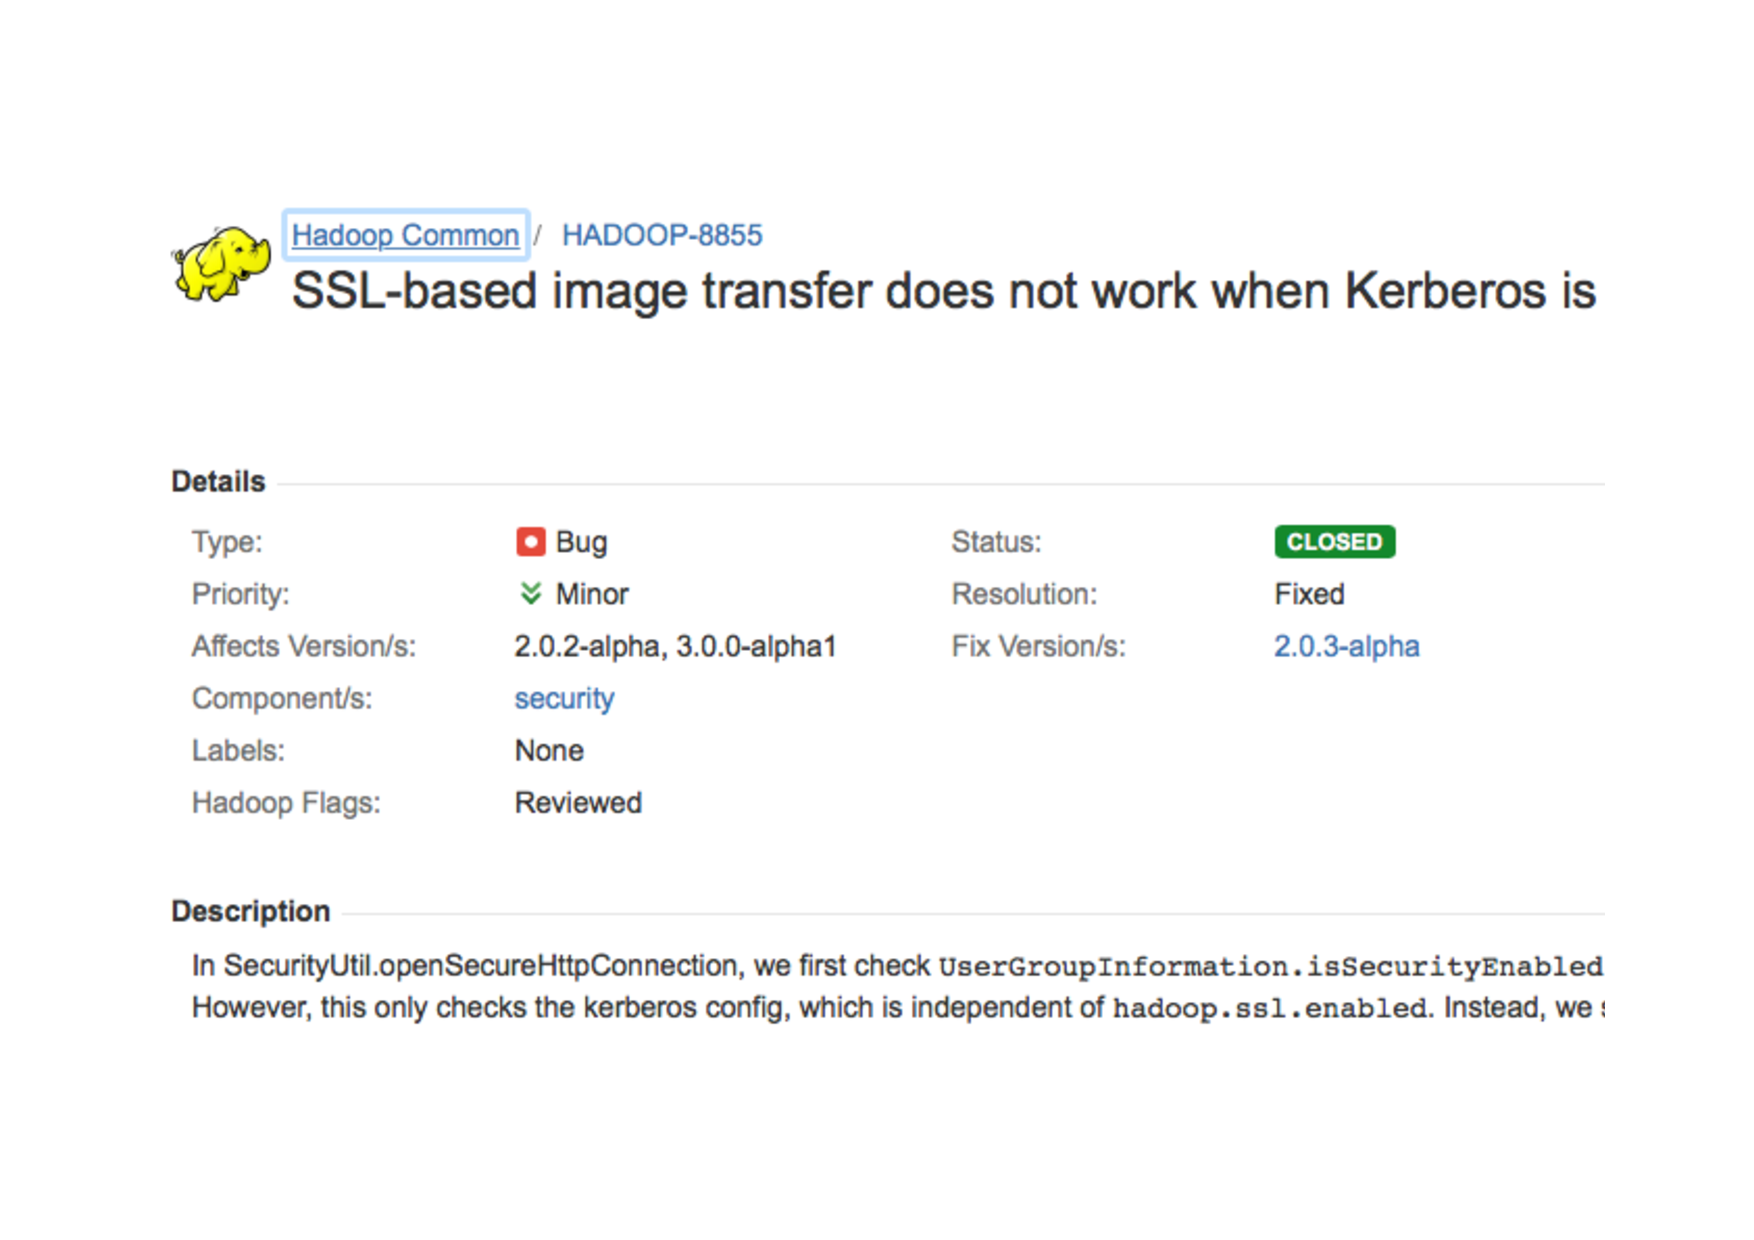
\includegraphics[width=1\textwidth]{figures/bug-report-example.pdf}
  \caption{A typical bug report (\url{https://issues.apache.org/jira/browse/HADOOP-8855}, as of September 2018)} 
  \label{fig:bug-report-example}
\end{figure}

\begin{figure}[!htp]
  \begin{subfigure}{.49\textwidth}
    \centering
    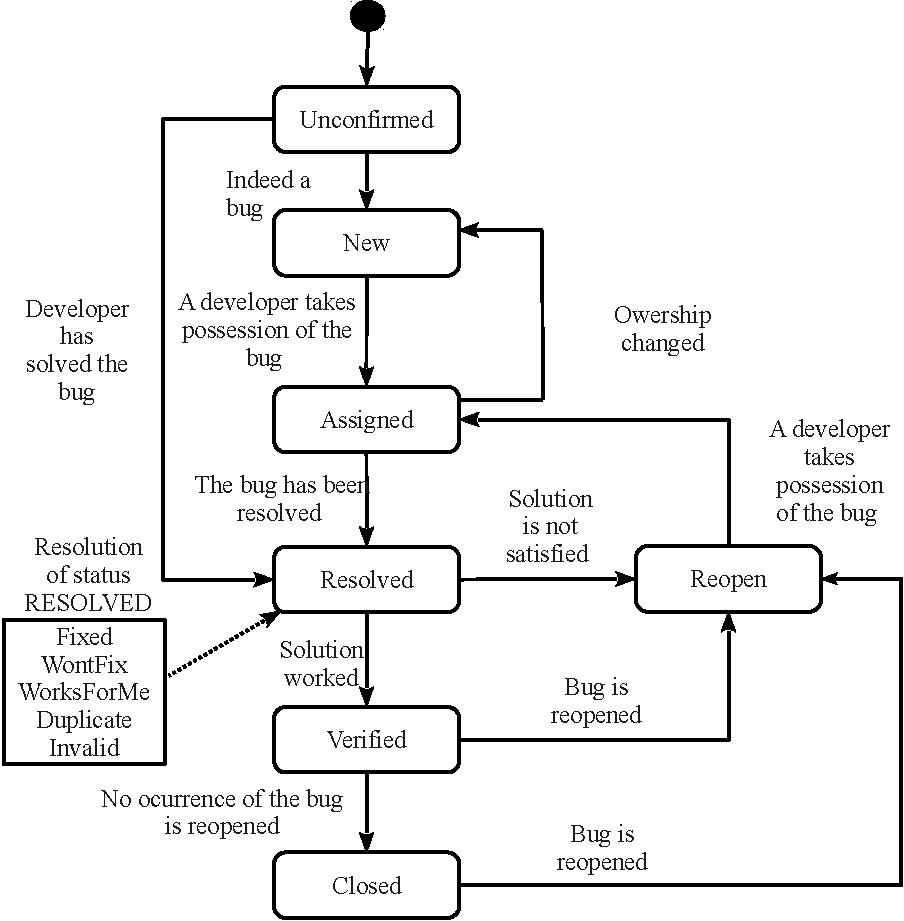
\includegraphics[width=\textwidth]{figures/bug-report-life-cycle.pdf}
    \caption{}
    \label{fig:life-cycle-of-bug-report}
  \end{subfigure}\hfill
  \begin{subfigure}{.40\textwidth}
    \centering
    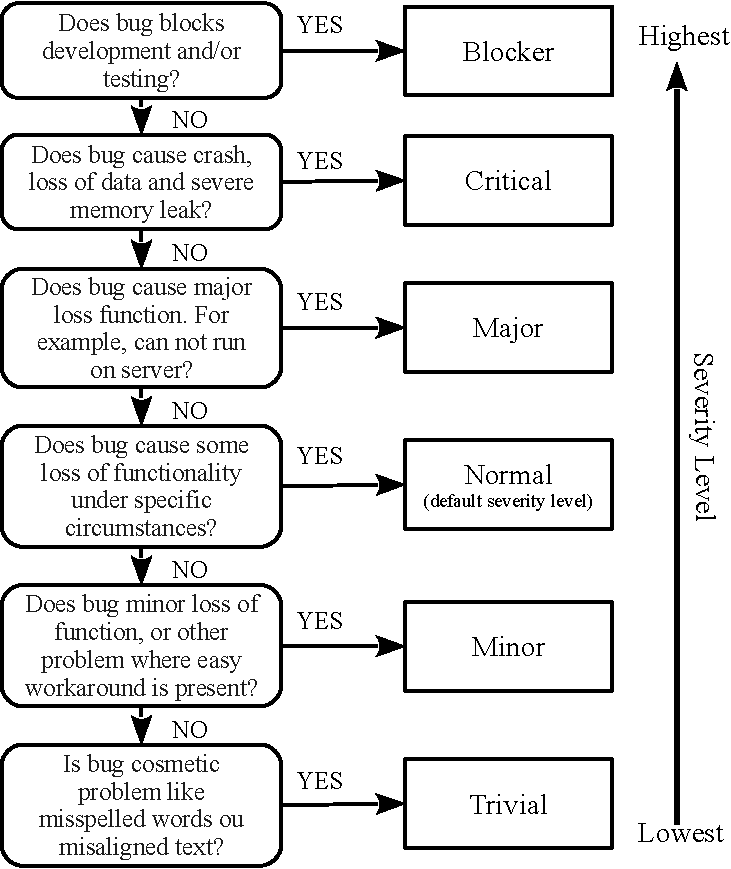
\includegraphics[width=\textwidth]{figures/bug-report-severity-levels.pdf}
    \caption{} 
    \label{fig:bug-report-severity-level-guideline}
  \end{subfigure}
  \caption{(a) The bug report lifecycle according to Zhang et al.\cite{Zhang:2015}. (b) Bugzilla guideline for bug report severity level assignment (\url{https://www.bugzilla.org}, as of \today).}
  \label{fig:bug-report-life-cycle-and-severity-level-guideline}
\end{figure}

Both users and development team members can define or redefine the severity level for a bug during the lifecycle. Figure \ref{fig:bug-report-severity-level-guideline} illustrates Bugzilla guidelines for assigning bug severity level. The Figure shows that such choices should be based on an affirmative answer to a question which characterizes a severity level appropriately. Also, the Figure indicates that \textit{Trivial} and \textit{Blocker} are lower and higher respectively.

To predict severity level, researchers sometimes aggregate these levels in severe (blocker, critical, and major) and non-severe (normal, minor and trivial) to work with a coarse-grained classification problem. Furthermore, some of them ignore the default severity level (often ``normal") because they consider this level as a choice made by users when they are not sure about the correct severity level. Other studies choose to predict a bug report severity level as \textit{blocking} or \textit{non-blocking} bug. A blocking bug is one that prevents other bugs to be fixed\cite{Valdivia:2014}. 

\subsection{Machine Learning}
Machine Learning (ML)\cite{Flach:2012} is an application of Artificial Intelligence (AI) that provides systems the ability to learn and improve from experience without being explicitly programmed. There are two types of ML algorithms: predictive (or supervised) and descriptive (or unsupervised). A predictive algorithm builds a model based on historical training data and uses this model to predict, from the values of input attributes, an output label (class attribute) for a new sample. A predictive task is called classification when the label value is discrete, or regression when the label value is continuous. 

On the other hand, a descriptive algorithm explores or describes a dataset. There is not an output label associated with a sample. Data clustering and pattern discovery are two examples of descriptive tasks. Bug report severity prediction is considered a classification problem; therefore, more detailing of descriptive algorithms are outside the scope of this paper.

\subsubsection{ML algorithms}
A ML algorithm works over a dataset, which contains many samples or instances $x_{i}$, where $i = \{1..n\}$. Each instance is composed of $\{x_{i1}, x_{i2},...,x_{id}\}$ input attributes or independent variables, where $d = \{1..m\}$, and one output attribute or dependent variable, $x_{i(m+1)}$.  Input attributes are commonly named features or feature vector, and output attribute as commonly named class or category. The most traditional ML classification algorithms are k-Nearest Neighbors, Näive Bayes, Decision Tree, Neural Networks, Random Forest and Support Vector Machine. In practice, they can be applied for both classification and regression tasks. However, this mapping review regards them only in the classification scenario. Next, a brief description of each one is presented\cite{Marsland:2014}:

\begin{itemize}
  \item \textbf{k-Nearest Neighbors} (k-NN) process the available instances (or neighbors) in a dataset and classifies a new instance based on its similarity measure to the k-nearest neighbors. Usually, k-NN algorithms utilize a Euclidean distance to quantify the proximity of neighbors. To calculate this distance, each feature vector of each instance in a dataset should represent a point of an n-dimensional space.
  
  \item \textbf{Näive Bayes} (NB) decides to which class an instance belongs based on the Bayesian Theorem of conditional probability. The probabilities of an instance belonging to each of the $C_{k}$ classes given the instance $x$ is $P(C_{k}|x )$. Näive Bayes classifiers assume that given the class variable, the value of a particular feature is independent of the value of any other feature.
  
  \item \textbf{Decision Tree} consists of a collection of internal nodes and leaf nodes in a tree, organized in a hierarchical model.  Each internal node represents a feature, and each leaf node corresponds to a class label. The decision tree classifiers organize a series of test questions and conditions in a tree structure.  A decision tree represents the model capable of guiding the decision making on the determination of the class to which an individual belongs.
  
  \item \textbf{Neural Network} is a learning algorithm that is inspired by the structure and functional aspects of biological neural networks\cite{Haykin:1998}. It structured as a network of units called neurons, with weighted, directed connections. Neural network models have been demonstrated to be capable of achieving remarkable performance in document classification\cite{Zhou:2012}.  \rem{Figure \ref{fig:artificial-neuron} presents an artificial neuron model that contains a set of weighted inputs ($w_i$), which corresponds to the synapses; an adder function ($\sum$) that sums the inputs signals; and an activation function ($f(.)$) that decides whether the neuron fires for the current inputs to generate the output value ($y_{o})$. Independent features of each instance represent neuron dendrites.}
  \rem{
  \begin{figure}[h!]
    \centering
    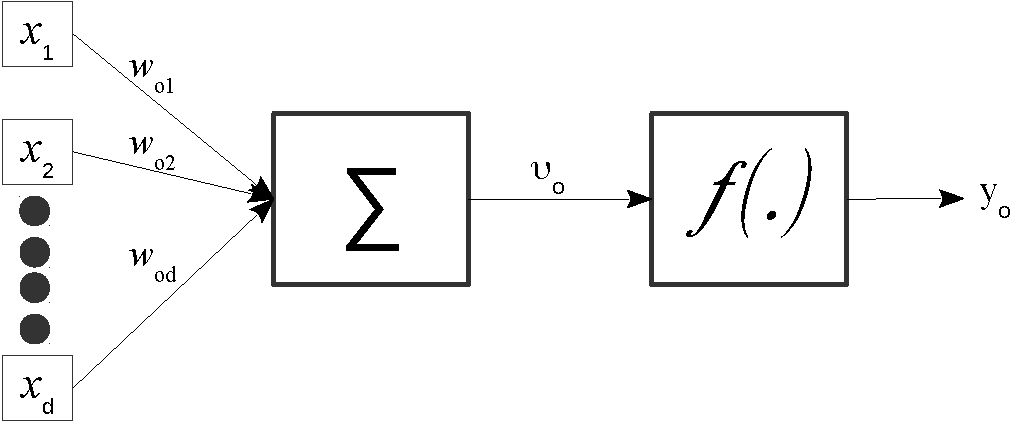
\includegraphics[width=0.5\textwidth]{figures/artificial-neuron.pdf}
    \caption{A artificial neuron model based on Marsland \cite{Marsland:2014}.}
    \label{fig:artificial-neuron}
  \end{figure}
  }
  \item \textbf{Support Vector Machine(SVM)}\rem{represents each feature vector of each instance as a point in an n-dimensional space. The algorithm divides every point belonging to a category in a particular space. Each space is separated by a gap that is as wide as possible\cite{Marsland:2014}. \rem{This space between these two regions delimits the margin between classes.}In Figure \ref{fig:support-vector-machine}, for example, SVM will search for support vectors which are instances located at the edge of an area in space. Such vectors define boundaries between one of these class instances (e.g., the crosses) and instances from another class (e.g., the circles).  \rem{Each region contains instances belonging to the same class\cite{Williams:2011}}. New instances are then mapped into that same space and predicted to belong to a category based on which side they are.}\edit{Each  feature vector of each instance is a point in an n-dimensional space.  SVM learns in this space an optimal way to separate the training instances according to their class labels. The output of this algorithm is a hyperplane, which maximizes the separation among feature vectors of instances of different classes. Given a new instance, SVM assigns a label based on which subspace  its feature vector belongs to~\cite{Tian:2016}.}
\rem{
  \begin{figure}[h!]
    \centering
    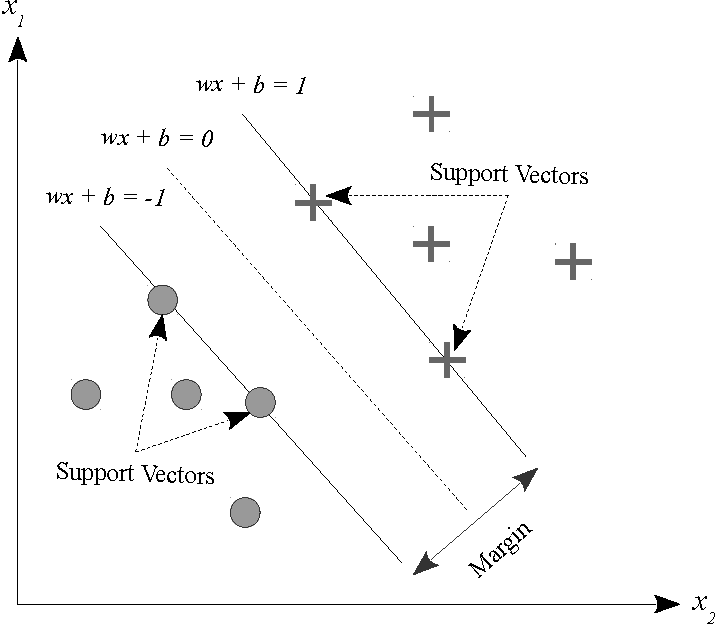
\includegraphics[width=0.4\textwidth]{figures/support-vector-machine.pdf}
    \caption{A SVM model example.}
    \label{fig:support-vector-machine}
  \end{figure}
}
  \item \textbf{Random Forest}\cite{Breiman:2001} relies on two core principles: (i) the creation of hundreds of decision trees and their combination into a single model; and (ii) the final decision is based on the ruling of the majority of the forming trees. 
\end{itemize}

\subsubsection{Feature Selection Methods}
Feature selection is the process of choosing a subset of features that better contribute to the accuracy of a predictive model. Three typical feature selection methods are described next\cite{Zheng:2004}:

\begin{itemize}
  \item \textbf{Information Gain (IG)}:  this method measures the number of bits of information obtained for category prediction by knowing the presence or absence of a feature in a dataset.
  \item \textbf{Chi-square (CHI)}: this method measures the lack of independence between a feature $f$ and category $c_i$ and can be compared to the chi-square distribution with one degree of freedom.
  \item \textbf{Correlation Coefficient (CC)}:  this method defines the correlation coefficient of feature $f$ with a category $c_i$.    
\end{itemize}

\subsubsection{Evaluation measures}
Accuracy, precision, recall, and F-measure are four measures commonly used to evaluate the performance of prediction models\cite{Feldman:2006}. The computation of the values of these measures are based on a \textit{confusion matrix}\cite{Williams:2011}, which represents the number of true/false positives, and the number of true/false negatives for each instance class value when making a prediction. Each measure is described next \cite{Japkowicz:2011}: 

\begin{itemize}
  \item \textbf{Accuracy} is the percentage of correctly classified observations among all observations:
  
  \begin{equation}
  Accuracy = \frac{TP+TN}{P+N}
  \end{equation}
  
  where P is the total of positive class instances, N is the total of negative class instances, TP is the number of true positives, and TN is the number of true negatives.
  
  \item \textbf{Precision} is the percentage of correctly classified observations among all observations that were assigned to the class by the classifier. It can be viewed as a measure of classifier exactness. A low precision can also indicate a large number of false positives. More formally recall is defined as:
  
  \begin{equation}
  Precision = \frac{TP}{TP+FP}
  \end{equation}
  
  where TP is the number of true positives, and FP is the number of false positives.
  
  \item \textbf{Recall} of a classification method can be defined as the percentage of correctly classified observations among all observations belonging to that class. It can be viewed as a measure of a classifiers completeness. A low recall indicates many false negatives in testing classification step. More formally recall is defined as: 
  
  \begin{equation}
  Recall = \frac{TP}{TP+FN}
  \end{equation}
  
  where TP is the number of true positives, and FN is the number of false negatives.
  
  \item \textbf{F-measure} is a harmonic mean of the precision and recall\cite{Feldman:2006}. F-measure can be calculated as:
  
  \begin{equation}
  \textit{F-measure} = \frac{2 \times (precision \times recall)}{(precision + recall)}
  \end{equation}
  
\end{itemize}

Receiving Operating Characteristics (ROC) is an alternative measure to evaluate binary classifiers. A ROC curve\cite{Japkowicz:2011} is a bidimensional chart, where the X-axis represents false positives, and the Y-axis represents true positives. The Area Under ROC Curve (AUC), ranging between 0 and 1, is used to assess the performance of ML algorithms. An algorithm outperforms another one if its AUC value is closer to 1. 

\subsubsection{Sampling methods}
The evaluation of the supervised method effectiveness is mainly based on two datasets with labeled samples, one for training the predictive model and the other for testing this model. Assessing performance of a predictive model using the same dataset for training and testing is not recommend and may yield misleading optimistic estimations\cite{Japkowicz:2011}. In order to obtain more reliable predictive estimates, resampling methods can be used to split the entire dataset into a training dataset and a testing dataset. Such methods according to  Facelli et al. \cite{Facelli:2015} include: 
\begin{itemize} 
  \item \textbf{Holdout} splits a dataset into a ratio of \textit{p} for training and $(1 - p)$ for testing. 
  \item \textbf{Cross-Validation (CV)} divides a dataset into $k$ folds. In each iteration, it saves a different fold for testing and uses all the others for training. 
  \item \textbf{Bootstrap} generates \textit{r} training subsets from the original dataset. It randomly samples instances with replacement from this set. Unselected cases make up the test subset. The result is the average performance observed for each test subset.
\end{itemize}

\subsubsection{Statistical tests}
\edit{Many scenarios require running several ML algorithms to chose the best predictive model. Even though the performance of these algorithms may be shown to be different on specific datasets, it needs to be confirmed whether the observed differences are statistically significant and not merely coincidental\cite{Japkowicz:2011}. In this situation, conducting statistical tests is a recommended practice for reliable comparison between predictive models under investigation\cite{Facelli:2015}. A brief description of four common statistical tests is provided:}

\begin{itemize}
  \item \textbf{T-Test}\cite{Japkowicz:2011} is a parametric statistical hypothesis test that can be used to assess whether the means of two groups are statistically different from each other.
  \item \textbf{Wilcoxon signed-rank test}\cite{Wilcoxon:1992} is a non-parametric statistical hypothesis test that can be used to determine whether two dependent samples, selected from the population, have the same distribution. 
  \item \textbf{Proportion test}\cite{Lewis:2013} is a parametric statistical hypothesis test that can be used to assess whether or not a sample from a population represents the true proportion of the entire population. 
  \item \textbf{Shapiro Wilk test}\cite{Lewis:2013} is a parametric statistical hypothesis test that can be used to test whether a sample $x_1, ..., x_n$ came from a normal distribution of the population.
\end{itemize}


\subsection{Text Mining}
The common ML algorithms cannot directly process unstructured text (e.g., \textit{summary} and \textit{description} fields from bug report form). Therefore, during a preprocessing step, these unstructured text fields are converted into more manageable representations. Typically, the content of these fields is represented by feature vectors, points of an n-dimensional space. Text mining is the process of converting unstructured text into a structure suited to analysis\cite{Feldman:2006}. It is composed of three primary activities\cite{Williams:2011}:

\begin{itemize}
  \item \textbf{Tokenization} is the action to parsing a character stream into a sequence of tokens by splitting the stream at delimiters. A token is a block of text or a string of characters (without delimiters such as spaces and punctuation), which is a useful portion of the unstructured data. 
  \item \textbf{Stop words removal} eliminates commonly used words that do not provide relevant information to a particular context, including prepositions, conjunctions, articles, common verbs, nouns, pronouns, adverbs, and adjectives. 
  \item \textbf{Stemming} is the process of reducing or normalizing inflected (or sometimes derived) words to their word stem, base form—generally a written word form (e.g., ``working” and ``worked" into ``work").
\end{itemize}

Two of the most traditional ways of representing a document relies on the use of a bag of words (unigrams) or a bag of bigrams (when two terms appear consecutively, one after the other)\cite{Feldman:2006}. In this approach all terms represent features, and thus the dimension of the feature space is equal to the number of different terms in all documents (bug reports). Methods for assigning weights to features may vary. The simplest one is to assign binary values representing the presence or absence of the term in each text. Term Frequency (TF), another type of quantification scheme, considers the number of times in which the term appears in each document. Term Frequency-Inverse Document Frequency (TD-IDF), a more complex type of scheme,  takes into account the frequencies of the term in each document, and in the whole collection.  The importance of a term in this scheme is proportional to its frequency in the document and inversely proportional to the frequency of the term in the collection. 
\section{Related Work}\label{sec:relatedwork} 

This section presents relevant articles in mining open system repositories, aiming at extracting data and using ML techniques to predict several maintenance properties. 

Menzies and Marcus\cite{Menzies2008} have developed a method, named SEVERIS (SEVERity ISsue assessment), for evaluating the severity of CRs. SEVERIS is based on established data and text mining techniques. The method was applied to predict CR severity level in five projects managed by the Project and Issue Tracking System (PITS), an issue tracker system used by NASA (Stratified F-measures by severity level in the range: (2) 78\%-86\%; (3) 68\%-98\%; (4) 86\%-92\%).


Lamkanfi et al.\cite{Lamkanfi2010} have developed an approach to predict if severity of bug report is non-severe (severity levels: 1 or 2) or severe (severity levels: 4 or 5) based on text mining algorithms (tokenization, stop word removal, stemming) and on the Naïve Bayes machine learning algorithm. They have validated their approach with data from three open source project (Mozilla, Eclipse, and GNOME). The article reports that a training set with approximately 500 CRs per severity level is sufficient to make predictions with reasonable accuracy (precision and recall in the range 0.65-0.75 with Mozilla and Eclipse; 0.70-0.85 with GNOME).

Valdivia et al.\cite{ValdiviaGarcia2014} have characterized blocking bugs in six open source projects and proposed a model to predict them. Their model was composed of 14 distinct factors or features (e.g. the textual description, location the bug is found in and the people involved with the bug). Based on these factors they have built decision trees for each project to predict whether a bug will be a blocking bug or not (F-measures in the range 15-42\%).

Tian et al.\cite{Tian2012} have develop a method to predict the severity level of new CRs based on similar CRs reported in the past. The comparison between old and new CRs was implemented by the BM25 similarity function. This method was applied to Mozilla, Eclipse and OpenOffice projects over more than 250,000 CR extracted from Bugzilla (F-measure in the range 13.9-65.3\% for Mozilla; 8.6-58\% for Eclipse; and 12.3-74\% for OpenOffice). 



\section{Research method}\label{sec:research_method}
This section describes the research method used in this mapping review for identifying and analyzing relevant papers. It is mainly based on the software engineering systematic literature review guidelines and recommendations proposed by Kitchenham et al.~\cite{Kitchenham:2007}, Brhel et al.~\cite{Brhel:2015}, Souza et al.~\cite{Desouza:2015}, and Petersen et al.~\cite{Petersen:2008}. These authors suggest a process with three main steps: planning, conducting, and reporting. In the planning step, they recommend defining a review protocol that includes a set of research questions, inclusion and exclusion criteria, sources of papers, search string, and mapping procedures. In the conducting step, they recommend selecting and retrieving papers for data extraction. Finally, in the reporting step, they recommend analyzing the results used to address research questions defined before.

\subsection{Research questions}\label{subsec:questions}
The main goal of this mapping review is to provide a current status of the research on bug report severity prediction in FLOSS. To ensure an unbiased selection process, this review addresses the following research questions.

\begin{enumerate}[label=\textbf{ RQ$_{\arabic*}$}., leftmargin=1.2cm]
  %% RQ1
  \item \textbf{When and where have the studies been published?} This research question gives to the researcher a perception whether the topic of this mapping review seems to be broad and new, providing an overview about where and when papers were published.
  
  %% RQ2
  \item \textbf{What FLOSS are the most used as report sources in experiments for bug report severity prediction?} This research question names the FLOSS used as report source in problems of bug report severity prediction. This overview can be useful for researchers that intend to accomplish new initiatives in this area, and can also motivate the adoption of new FLOSS in future research to bridge existing gaps.
  
  %% RQ3
  \item \textbf{Was bug report severity prediction most addressed as either a fine-grained label  or coarse-grained label prediction problem?} This research question investigates whether bug report severity prediction was handled as a fine-grained label (i.e., multi-label) or as a coarse-grained label (i.e., two-label or three-label) prediction problem. Understanding each solution provided for each prediction problem type is essential for guiding the selection of suitable machine learning algorithm.
  
  %% RQ4
  \item \textbf{What are the most common features used for bug report severity prediction?} This question investigates features used for bug report severity prediction in FLOSS. It can help to map which features have been considered more effective for this prediction problem.
  
  %% RQ5
  \item \textbf{What are the most common feature selection methods used for bug report severity prediction?} This question complements the previous one, looking for feature selection methods employed in the papers for bug report severity prediction in FLOSS. Also, this RQ allows for identifying which feature selection approaches have been considered more suitable for this prediction problem.
  
  %% RQ6
  \item \textbf{What are the most used text mining or information retrieval methods for bug report severity prediction?} This research question indicates the main text mining approaches used to extract features from textual fields of bug reports. It can guide researchers in the task of selecting text mining methods more suitable to be applied in bug report severity prediction or similar problems. 
  
  %% RQ7    
  \item \textbf{What are the most used machine learning algorithms for bug report severity prediction?} This research question aims to identify the main ML algorithms, which have been adopted for bug report severity prediction in FLOSS. Also, this RQ can be useful for any researcher that intends to accomplish further initiatives in this area, as well as to guide him/her in search of other algorithms to advance the state of the art.
  
  %% RQ8
  \item \textbf{What are the measures typically used to evaluate ML algorithms performance for bug report severity prediction?} This research question aims to find out which measures are used to evaluate ML algorithms performance. It can be helpful to identify the more appropriate measures to evaluate ML algorithms performance for bug report severity prediction. 
  
  %% RQ9   
  \item \textbf{Which sampling techniques are applied most frequently to generate more reliable predictive performance estimates in severity prediction of a bug report?} This question complements the previous one, investigating sampling techniques, which have been used to generate more reliable and accurate ML models. It can be useful to analyze sampling techniques, which might be more suitable to improve machine learning algorithms performance for bug report severity prediction.
  
  %% RQ10
  \item \textbf{Which statistical tests were used to compare the performance between two or more ML algorithms for bug report severity prediction?} The answer to this research question can be useful to identify which statistical tests were used in the context of bug report severity prediction. In addition, it allows grasping existing protocols for the comparison between two or more ML algorithms performance using statistical significance tests.
  
  %% RQ11 
  \item \textbf{Which software tools were used to run experiments for bug report severity prediction?} This research question highlights the software tools most used to run experiments for bug reports severity prediction in FLOSS projects. It is useful to provide information for researchers and practitioners about technologies that could be used in their experiments.
  
  %% RQ12
  \item \textbf{Which solution types were proposed for the problem of bug report severity prediction?} This research question examines whether the most common solutions proposed in the selected studies are either online or off-line. This is important to separate the solutions that can be applied only in an experimental environment (off-line) from those that also can be deployed in a real scenario (online).
\end{enumerate}

\subsection{Paper selection}\label{subsec:selection}
This section describes the selection process carried out through this systematic mapping review. It comprises four steps: (i) terms and searching string; (ii) sources for searching; (iii) inclusion and exclusion criteria; and (iv) data storage procedures.

\subsubsection{Terms and search string}\label{subsubsec:string}
The base string was constructed from three main search terms related to three distinct knowledge areas: ``open source project", ``bug report" and ``severity predict." To build the search string, terms were combined with ``AND" connectors. The search string syntax was adapted according to particularities of each source (e.g., wildcards, connectors, apostrophes, and quotation marks) before it has been applied on three metadata papers: title, abstract, and keywords. Table~\ref{tab:search_string} exhibits terms and final search string used in this systematic mapping review.

\begin{table*}[ht!]
  \centering
  \spacebtrows{1.3}
  \caption{Search string.}
  \begin{tabular}{@{}ll@{}} 
    \toprule
    \textbf{Area} & \textbf{Search term}\\ 
    \midrule
    Bug report & ``bug report"\\ 
    Open source & ``open source software" \\
    Severity prediction & ``severity predict"\\ 
    \midrule
    \textbf{Search string}: & ``open source software" AND ``severity predict" AND ``bug report"\\ 
    \bottomrule
  \end{tabular}
  \label{tab:search_string}
\end{table*}

\subsubsection{Sources}\label{subsubsec:sources}
To accomplish this systematic mapping review, four electronic databases and one popular search engines were selected, as recommended by Kitchenham et al.~\cite{Kitchenham:2007}. Table~\ref{tab:search_sources} shows each selected search sources, as well as the search date, and the period covered by the search. 

\begin{table*}[!htbp]
  \centering
  %\spacebtrows{1.3}
  \caption{Search sources.}
  \begin{tabular}{@{}lllll@{}} 
    \toprule
    \textbf{Source} & \textbf{Electronic address} & \textbf{Type} & \textbf{Search Date} & \textbf{Years covered}\\ 
    \midrule
    ACM              &  \url{http://dl.acm.og}     & Digital library   & Dec,17 & 2010 - 2017\\ 
    IEEE             &  \url{http://ieeexplore.ieee.org}               & Digital library   & Dec,17 & 2010 - 2017\\ 
    Google Scholar   &  \url{http://www.scholar.google.com}  & Search engine     & Dec,17 & 2010 - 2017\\ 
    Science Direct   &  \url{http://www.sciencedirect.com}   & Digital library   & Dec,17 & 2010 - 2017\\
    SpringLink       &  \url{http://www.springerlink.com}    & Digital library   & Dec,17 & 2010 - 2017\\
    \bottomrule
  \end{tabular}
  \label{tab:search_sources}
\end{table*}

\subsubsection{Inclusion and exclusion criteria}\label{subsubsec:criteria}
The inclusion criteria below allow the identification of papers in the existing literature.

\begin{center}
  \begin{enumerate}[label=\textbf{ IC$_\arabic*$}., leftmargin=1.1cm]
    \item The paper discusses bug report severity prediction in FLOSS projects.
  \end{enumerate}
\end{center}

On the contrary, the following exclusion criteria allow excluding all papers that satisfy any of them.

\begin{enumerate}[label=\textbf{ EC$_\arabic*$}., leftmargin=1.1cm]
  \item The paper does not have an abstract;
  \item The paper is just published as an abstract;
  \item The paper is written in a language other than English;
  \item The paper is not a primary paper (e.g., keynotes);
  \item The paper is not accessible on the Web;
\end{enumerate}

\subsubsection{Data storage}\label{subsubsec:storage}
The data extracted in the searching phase were stored into a spreadsheet that recorded all relevant details from selected papers. This spreadsheet supported classification and analysis procedures throughout this systematic mapping review.

\subsubsection{Assessment}\label{subsubsec:assessment}
According to Kitchenham et al.~\cite{Kitchenham:2007}, the consistency of the protocol utilized in a systematic mapping  should be reviewed to confirm that: ``the search strings, constructed interactively, derived from the research questions";  ``the data to be extracted will properly address the research question(s)"; ``the data analysis procedure is appropriate to answer the research questions". In this research, the first author is a Ph.D. candidate running the experiments. The second and third authors conducted the review process.

\subsection{Data extraction and synthesis}\label{subsec:extraction}

Figure~\ref{fig:smr_selection_phases} illustrates the four-stage selection process carried out in the current mapping review. In each stage, the sample size was reduced based on the inclusion and exclusion criteria. In the first stage, relevant papers were retrieved by querying the databases with the search string presented in Table~\ref{tab:search_string}. All database queries were issued in December 2017. This yielded a total of 54 initial papers: 13 from \textbf{IEEE Xplore}, 5 from \textbf{Science Direct}, 17 from \textbf{ACM Digital Library}, and 19 from \textbf{SpringerLink}. After removing four duplicates, we reduced (around 7\%) the initial set of 50 papers. 
In the second stage, inclusion and exclusion criteria were applied over title, abstract, and keywords, reaching a set of 18 papers (reduction around 64\%): 32 papers were rejected for not satisfying IC$_{1}$ (The paper discusses severity prediction of bug reports in FLOSS projects). In the third stage, exclusion criteria were applied considering the full text. However, no paper was rejected by taking into account these criteria. 

In the fourth stage, the Snowballing (search for references)~\cite{Kitchenham:2007} activity was conducted, which resulted in 12 additional papers. After applying selection criteria over title, abstract, and keywords, 11 papers remained (reduction of 8.3\% over the papers selected by snowballing). For these papers, selection criteria were applied considering the full text, and nine papers remained (reduction of approximately 18.2\% over the 11 previously selected papers); EC$_{3}$ criterion eliminated one paper (the paper is  written in a language other than English); EC$_{6}$ eliminated one more paper (the paper is not accessible on the Web), and another one  was rejected for not satisfying IC$_{1}$. The selection phase ended up with 27 papers to be analyzed (18 from the sources plus nine from snowballing). Table~\ref{tab:selected_studies} shows the bibliographic reference of selected papers and an reference identifier (ID) for each paper. Throughout the remainder of this text, these identifiers will be used to refer to the corresponding paper.

\begin{figure}[h!]
  \centering
  %% Graphic for TeX using PGF
% Title: /home/luiz/study-selection-phases.dia
% Creator: Dia v0.97.3
% CreationDate: Thu May 24 22:14:20 2018
% For: luiz
% \usepackage{tikz}
% The following commands are not supported in PSTricks at present
% We define them conditionally, so when they are implemented,
% this pgf file will use them.
\ifx\du\undefined
  \newlength{\du}
\fi
\setlength{\du}{15\unitlength}
\begin{tikzpicture}
\pgftransformxscale{1.000000}
\pgftransformyscale{-1.000000}
\definecolor{dialinecolor}{rgb}{0.000000, 0.000000, 0.000000}
\pgfsetstrokecolor{dialinecolor}
\definecolor{dialinecolor}{rgb}{1.000000, 1.000000, 1.000000}
\pgfsetfillcolor{dialinecolor}
\definecolor{dialinecolor}{rgb}{1.000000, 1.000000, 1.000000}
\pgfsetfillcolor{dialinecolor}
\fill (-31.917258\du,3.529206\du)--(-31.917258\du,6.807243\du)--(-19.614266\du,6.807243\du)--(-19.614266\du,3.529206\du)--cycle;
\pgfsetlinewidth{0.090000\du}
\pgfsetdash{}{0pt}
\pgfsetdash{}{0pt}
\pgfsetmiterjoin
\definecolor{dialinecolor}{rgb}{0.301961, 0.301961, 0.301961}
\pgfsetstrokecolor{dialinecolor}
\draw (-31.917258\du,3.529206\du)--(-31.917258\du,6.807243\du)--(-19.614266\du,6.807243\du)--(-19.614266\du,3.529206\du)--cycle;
% setfont left to latex
\definecolor{dialinecolor}{rgb}{0.000000, 0.000000, 0.000000}
\pgfsetstrokecolor{dialinecolor}
\node at (-25.765762\du,5.249336\du){};
\definecolor{dialinecolor}{rgb}{1.000000, 1.000000, 1.000000}
\pgfsetfillcolor{dialinecolor}
\fill (-31.448657\du,4.108500\du)--(-31.448657\du,6.196277\du)--(-29.033657\du,6.196277\du)--(-29.033657\du,4.108500\du)--cycle;
\pgfsetlinewidth{0.090000\du}
\pgfsetdash{}{0pt}
\pgfsetdash{}{0pt}
\pgfsetmiterjoin
\definecolor{dialinecolor}{rgb}{0.301961, 0.301961, 0.301961}
\pgfsetstrokecolor{dialinecolor}
\draw (-31.448657\du,4.108500\du)--(-31.448657\du,6.196277\du)--(-29.033657\du,6.196277\du)--(-29.033657\du,4.108500\du)--cycle;
% setfont left to latex
\definecolor{dialinecolor}{rgb}{0.000000, 0.000000, 0.000000}
\pgfsetstrokecolor{dialinecolor}
\node at (-30.241157\du,5.075166\du){\tiny Springer Link};
% setfont left to latex
\definecolor{dialinecolor}{rgb}{0.000000, 0.000000, 0.000000}
\pgfsetstrokecolor{dialinecolor}
\node at (-30.241157\du,5.357389\du){\tiny (19 papers)};
\definecolor{dialinecolor}{rgb}{1.000000, 1.000000, 1.000000}
\pgfsetfillcolor{dialinecolor}
\fill (-28.859928\du,4.108500\du)--(-28.859928\du,6.196277\du)--(-25.689668\du,6.196277\du)--(-25.689668\du,4.108500\du)--cycle;
\pgfsetlinewidth{0.090000\du}
\pgfsetdash{}{0pt}
\pgfsetdash{}{0pt}
\pgfsetmiterjoin
\definecolor{dialinecolor}{rgb}{0.301961, 0.301961, 0.301961}
\pgfsetstrokecolor{dialinecolor}
\draw (-28.859928\du,4.108500\du)--(-28.859928\du,6.196277\du)--(-25.689668\du,6.196277\du)--(-25.689668\du,4.108500\du)--cycle;
% setfont left to latex
\definecolor{dialinecolor}{rgb}{0.000000, 0.000000, 0.000000}
\pgfsetstrokecolor{dialinecolor}
\node at (-27.274798\du,5.075166\du){\tiny ACM Digital Library};
% setfont left to latex
\definecolor{dialinecolor}{rgb}{0.000000, 0.000000, 0.000000}
\pgfsetstrokecolor{dialinecolor}
\node at (-27.274798\du,5.357389\du){\tiny (19 papers)};
% setfont left to latex
\definecolor{dialinecolor}{rgb}{0.000000, 0.000000, 0.000000}
\pgfsetstrokecolor{dialinecolor}
\node[anchor=west] at (-27.274798\du,5.152389\du){};
\definecolor{dialinecolor}{rgb}{1.000000, 1.000000, 1.000000}
\pgfsetfillcolor{dialinecolor}
\fill (-25.520498\du,4.108500\du)--(-25.520498\du,6.196277\du)--(-23.205498\du,6.196277\du)--(-23.205498\du,4.108500\du)--cycle;
\pgfsetlinewidth{0.090000\du}
\pgfsetdash{}{0pt}
\pgfsetdash{}{0pt}
\pgfsetmiterjoin
\definecolor{dialinecolor}{rgb}{0.301961, 0.301961, 0.301961}
\pgfsetstrokecolor{dialinecolor}
\draw (-25.520498\du,4.108500\du)--(-25.520498\du,6.196277\du)--(-23.205498\du,6.196277\du)--(-23.205498\du,4.108500\du)--cycle;
% setfont left to latex
\definecolor{dialinecolor}{rgb}{0.000000, 0.000000, 0.000000}
\pgfsetstrokecolor{dialinecolor}
\node at (-24.362998\du,5.075166\du){\tiny IEEE Xplore};
% setfont left to latex
\definecolor{dialinecolor}{rgb}{0.000000, 0.000000, 0.000000}
\pgfsetstrokecolor{dialinecolor}
\node at (-24.362998\du,5.357389\du){\tiny (13 papers)};
\definecolor{dialinecolor}{rgb}{1.000000, 1.000000, 1.000000}
\pgfsetfillcolor{dialinecolor}
\fill (-22.986880\du,4.108500\du)--(-22.986880\du,6.196277\du)--(-20.079380\du,6.196277\du)--(-20.079380\du,4.108500\du)--cycle;
\pgfsetlinewidth{0.090000\du}
\pgfsetdash{}{0pt}
\pgfsetdash{}{0pt}
\pgfsetmiterjoin
\definecolor{dialinecolor}{rgb}{0.301961, 0.301961, 0.301961}
\pgfsetstrokecolor{dialinecolor}
\draw (-22.986880\du,4.108500\du)--(-22.986880\du,6.196277\du)--(-20.079380\du,6.196277\du)--(-20.079380\du,4.108500\du)--cycle;
% setfont left to latex
\definecolor{dialinecolor}{rgb}{0.000000, 0.000000, 0.000000}
\pgfsetstrokecolor{dialinecolor}
\node at (-21.533130\du,5.057111\du){\tiny Science Direct};
% setfont left to latex
\definecolor{dialinecolor}{rgb}{0.000000, 0.000000, 0.000000}
\pgfsetstrokecolor{dialinecolor}
\node at (-21.533130\du,5.409889\du){\tiny (13 papers)};
\definecolor{dialinecolor}{rgb}{1.000000, 1.000000, 1.000000}
\pgfsetfillcolor{dialinecolor}
\fill (-16.409595\du,3.197689\du)--(-16.409595\du,7.093022\du)--(-6.750481\du,7.093022\du)--(-6.750481\du,3.197689\du)--cycle;
\pgfsetlinewidth{0.090000\du}
\pgfsetdash{}{0pt}
\pgfsetdash{}{0pt}
\pgfsetmiterjoin
\definecolor{dialinecolor}{rgb}{0.301961, 0.301961, 0.301961}
\pgfsetstrokecolor{dialinecolor}
\draw (-16.409595\du,3.197689\du)--(-16.409595\du,7.093022\du)--(-6.750481\du,7.093022\du)--(-6.750481\du,3.197689\du)--cycle;
% setfont left to latex
\definecolor{dialinecolor}{rgb}{0.000000, 0.000000, 0.000000}
\pgfsetstrokecolor{dialinecolor}
\node at (-11.580038\du,4.168133\du){};
% setfont left to latex
\definecolor{dialinecolor}{rgb}{0.000000, 0.000000, 0.000000}
\pgfsetstrokecolor{dialinecolor}
\node at (-11.580038\du,4.520911\du){};
% setfont left to latex
\definecolor{dialinecolor}{rgb}{0.000000, 0.000000, 0.000000}
\pgfsetstrokecolor{dialinecolor}
\node at (-11.580038\du,4.873689\du){};
% setfont left to latex
\definecolor{dialinecolor}{rgb}{0.000000, 0.000000, 0.000000}
\pgfsetstrokecolor{dialinecolor}
\node at (-11.580038\du,5.226466\du){};
% setfont left to latex
\definecolor{dialinecolor}{rgb}{0.000000, 0.000000, 0.000000}
\pgfsetstrokecolor{dialinecolor}
\node at (-11.580038\du,5.579244\du){};
% setfont left to latex
\definecolor{dialinecolor}{rgb}{0.000000, 0.000000, 0.000000}
\pgfsetstrokecolor{dialinecolor}
\node at (-11.580038\du,5.932022\du){};
% setfont left to latex
\definecolor{dialinecolor}{rgb}{0.000000, 0.000000, 0.000000}
\pgfsetstrokecolor{dialinecolor}
\node at (-11.580038\du,6.284800\du){};
% setfont left to latex
\definecolor{dialinecolor}{rgb}{0.000000, 0.000000, 0.000000}
\pgfsetstrokecolor{dialinecolor}
\node[anchor=west] at (-14.727183\du,10.833293\du){};
% setfont left to latex
\definecolor{dialinecolor}{rgb}{0.000000, 0.000000, 0.000000}
\pgfsetstrokecolor{dialinecolor}
\node[anchor=west] at (-11.580038\du,5.145355\du){};
\definecolor{dialinecolor}{rgb}{1.000000, 1.000000, 1.000000}
\pgfsetfillcolor{dialinecolor}
\fill (-16.409595\du,8.014929\du)--(-16.409595\du,11.574374\du)--(-6.787316\du,11.574374\du)--(-6.787316\du,8.014929\du)--cycle;
\pgfsetlinewidth{0.090000\du}
\pgfsetdash{}{0pt}
\pgfsetdash{}{0pt}
\pgfsetmiterjoin
\definecolor{dialinecolor}{rgb}{0.301961, 0.301961, 0.301961}
\pgfsetstrokecolor{dialinecolor}
\draw (-16.409595\du,8.014929\du)--(-16.409595\du,11.574374\du)--(-6.787316\du,11.574374\du)--(-6.787316\du,8.014929\du)--cycle;
% setfont left to latex
\definecolor{dialinecolor}{rgb}{0.000000, 0.000000, 0.000000}
\pgfsetstrokecolor{dialinecolor}
\node at (-11.598455\du,8.817429\du){};
% setfont left to latex
\definecolor{dialinecolor}{rgb}{0.000000, 0.000000, 0.000000}
\pgfsetstrokecolor{dialinecolor}
\node at (-11.598455\du,9.170207\du){};
% setfont left to latex
\definecolor{dialinecolor}{rgb}{0.000000, 0.000000, 0.000000}
\pgfsetstrokecolor{dialinecolor}
\node at (-11.598455\du,9.522985\du){};
% setfont left to latex
\definecolor{dialinecolor}{rgb}{0.000000, 0.000000, 0.000000}
\pgfsetstrokecolor{dialinecolor}
\node at (-11.598455\du,9.875763\du){};
% setfont left to latex
\definecolor{dialinecolor}{rgb}{0.000000, 0.000000, 0.000000}
\pgfsetstrokecolor{dialinecolor}
\node at (-11.598455\du,10.228540\du){};
% setfont left to latex
\definecolor{dialinecolor}{rgb}{0.000000, 0.000000, 0.000000}
\pgfsetstrokecolor{dialinecolor}
\node at (-11.598455\du,10.581318\du){};
% setfont left to latex
\definecolor{dialinecolor}{rgb}{0.000000, 0.000000, 0.000000}
\pgfsetstrokecolor{dialinecolor}
\node at (-11.598455\du,10.934096\du){};
% setfont left to latex
\definecolor{dialinecolor}{rgb}{0.000000, 0.000000, 0.000000}
\pgfsetstrokecolor{dialinecolor}
\node[anchor=west] at (-11.598455\du,9.794652\du){};
% setfont left to latex
\definecolor{dialinecolor}{rgb}{0.000000, 0.000000, 0.000000}
\pgfsetstrokecolor{dialinecolor}
\node[anchor=west] at (-12.122732\du,8.459829\du){};
% setfont left to latex
\definecolor{dialinecolor}{rgb}{0.000000, 0.000000, 0.000000}
\pgfsetstrokecolor{dialinecolor}
\node[anchor=west] at (-15.897732\du,9.584829\du){};
% setfont left to latex
\definecolor{dialinecolor}{rgb}{0.000000, 0.000000, 0.000000}
\pgfsetstrokecolor{dialinecolor}
\node[anchor=west] at (-12.154697\du,8.372549\du){};
% setfont left to latex
\definecolor{dialinecolor}{rgb}{0.000000, 0.000000, 0.000000}
\pgfsetstrokecolor{dialinecolor}
\node[anchor=west] at (-11.598455\du,9.794652\du){};
% setfont left to latex
\definecolor{dialinecolor}{rgb}{0.000000, 0.000000, 0.000000}
\pgfsetstrokecolor{dialinecolor}
\node[anchor=west] at (-12.974637\du,7.860073\du){};
% setfont left to latex
\definecolor{dialinecolor}{rgb}{0.000000, 0.000000, 0.000000}
\pgfsetstrokecolor{dialinecolor}
\node[anchor=west] at (-14.979697\du,8.522549\du){};
% setfont left to latex
\definecolor{dialinecolor}{rgb}{0.000000, 0.000000, 0.000000}
\pgfsetstrokecolor{dialinecolor}
\node[anchor=west] at (-10.466532\du,8.591129\du){};
\definecolor{dialinecolor}{rgb}{1.000000, 1.000000, 1.000000}
\pgfsetfillcolor{dialinecolor}
\fill (-23.887162\du,8.059949\du)--(-23.887162\du,11.619393\du)--(-19.569166\du,11.619393\du)--(-19.569166\du,8.059949\du)--cycle;
\pgfsetlinewidth{0.090000\du}
\pgfsetdash{}{0pt}
\pgfsetdash{}{0pt}
\pgfsetmiterjoin
\definecolor{dialinecolor}{rgb}{0.301961, 0.301961, 0.301961}
\pgfsetstrokecolor{dialinecolor}
\draw (-23.887162\du,8.059949\du)--(-23.887162\du,11.619393\du)--(-19.569166\du,11.619393\du)--(-19.569166\du,8.059949\du)--cycle;
% setfont left to latex
\definecolor{dialinecolor}{rgb}{0.000000, 0.000000, 0.000000}
\pgfsetstrokecolor{dialinecolor}
\node at (-21.728164\du,8.862449\du){};
% setfont left to latex
\definecolor{dialinecolor}{rgb}{0.000000, 0.000000, 0.000000}
\pgfsetstrokecolor{dialinecolor}
\node at (-21.728164\du,9.215226\du){};
% setfont left to latex
\definecolor{dialinecolor}{rgb}{0.000000, 0.000000, 0.000000}
\pgfsetstrokecolor{dialinecolor}
\node at (-21.728164\du,9.568004\du){};
% setfont left to latex
\definecolor{dialinecolor}{rgb}{0.000000, 0.000000, 0.000000}
\pgfsetstrokecolor{dialinecolor}
\node at (-21.728164\du,9.920782\du){};
% setfont left to latex
\definecolor{dialinecolor}{rgb}{0.000000, 0.000000, 0.000000}
\pgfsetstrokecolor{dialinecolor}
\node at (-21.728164\du,10.273560\du){};
% setfont left to latex
\definecolor{dialinecolor}{rgb}{0.000000, 0.000000, 0.000000}
\pgfsetstrokecolor{dialinecolor}
\node at (-21.728164\du,10.626338\du){};
% setfont left to latex
\definecolor{dialinecolor}{rgb}{0.000000, 0.000000, 0.000000}
\pgfsetstrokecolor{dialinecolor}
\node at (-21.728164\du,10.979115\du){};
% setfont left to latex
\definecolor{dialinecolor}{rgb}{0.000000, 0.000000, 0.000000}
\pgfsetstrokecolor{dialinecolor}
\node[anchor=west] at (-21.728164\du,9.839671\du){};
% setfont left to latex
\definecolor{dialinecolor}{rgb}{0.000000, 0.000000, 0.000000}
\pgfsetstrokecolor{dialinecolor}
\node[anchor=west] at (-22.296676\du,9.004456\du){\scriptsize \textbf{Stage 3}};
% setfont left to latex
\definecolor{dialinecolor}{rgb}{0.000000, 0.000000, 0.000000}
\pgfsetstrokecolor{dialinecolor}
\node[anchor=west] at (-17.469006\du,11.002467\du){};
% setfont left to latex
\definecolor{dialinecolor}{rgb}{0.000000, 0.000000, 0.000000}
\pgfsetstrokecolor{dialinecolor}
\node[anchor=west] at (-22.385901\du,10.417810\du){};
% setfont left to latex
\definecolor{dialinecolor}{rgb}{0.000000, 0.000000, 0.000000}
\pgfsetstrokecolor{dialinecolor}
\node[anchor=west] at (-21.728164\du,9.839671\du){};
% setfont left to latex
\definecolor{dialinecolor}{rgb}{0.000000, 0.000000, 0.000000}
\pgfsetstrokecolor{dialinecolor}
\node[anchor=west] at (-30.104804\du,11.393752\du){};
% setfont left to latex
\definecolor{dialinecolor}{rgb}{0.000000, 0.000000, 0.000000}
\pgfsetstrokecolor{dialinecolor}
\node[anchor=west] at (-26.271407\du,8.805627\du){};
% setfont left to latex
\definecolor{dialinecolor}{rgb}{0.000000, 0.000000, 0.000000}
\pgfsetstrokecolor{dialinecolor}
\node[anchor=west] at (-21.985901\du,10.425310\du){};
\pgfsetlinewidth{0.100000\du}
\pgfsetdash{}{0pt}
\pgfsetdash{}{0pt}
\pgfsetbuttcap
\pgfsetmiterjoin
\pgfsetlinewidth{0.100000\du}
\pgfsetbuttcap
\pgfsetmiterjoin
\pgfsetdash{}{0pt}
\definecolor{dialinecolor}{rgb}{1.000000, 1.000000, 1.000000}
\pgfsetfillcolor{dialinecolor}
\pgfpathmoveto{\pgfpoint{-14.364235\du}{4.109362\du}}
\pgfpathlineto{\pgfpoint{-8.656319\du}{4.109362\du}}
\pgfpathcurveto{\pgfpoint{-7.868219\du}{4.109362\du}}{\pgfpoint{-7.229340\du}{4.358800\du}}{\pgfpoint{-7.229340\du}{4.666496\du}}
\pgfpathcurveto{\pgfpoint{-7.229340\du}{4.974193\du}}{\pgfpoint{-7.868219\du}{5.223630\du}}{\pgfpoint{-8.656319\du}{5.223630\du}}
\pgfpathlineto{\pgfpoint{-14.364235\du}{5.223630\du}}
\pgfpathcurveto{\pgfpoint{-15.152334\du}{5.223630\du}}{\pgfpoint{-15.791214\du}{4.974193\du}}{\pgfpoint{-15.791214\du}{4.666496\du}}
\pgfpathcurveto{\pgfpoint{-15.791214\du}{4.358800\du}}{\pgfpoint{-15.152334\du}{4.109362\du}}{\pgfpoint{-14.364235\du}{4.109362\du}}
\pgfusepath{fill}
\definecolor{dialinecolor}{rgb}{0.301961, 0.301961, 0.301961}
\pgfsetstrokecolor{dialinecolor}
\pgfpathmoveto{\pgfpoint{-14.364235\du}{4.109362\du}}
\pgfpathlineto{\pgfpoint{-8.656319\du}{4.109362\du}}
\pgfpathcurveto{\pgfpoint{-7.868219\du}{4.109362\du}}{\pgfpoint{-7.229340\du}{4.358800\du}}{\pgfpoint{-7.229340\du}{4.666496\du}}
\pgfpathcurveto{\pgfpoint{-7.229340\du}{4.974193\du}}{\pgfpoint{-7.868219\du}{5.223630\du}}{\pgfpoint{-8.656319\du}{5.223630\du}}
\pgfpathlineto{\pgfpoint{-14.364235\du}{5.223630\du}}
\pgfpathcurveto{\pgfpoint{-15.152334\du}{5.223630\du}}{\pgfpoint{-15.791214\du}{4.974193\du}}{\pgfpoint{-15.791214\du}{4.666496\du}}
\pgfpathcurveto{\pgfpoint{-15.791214\du}{4.358800\du}}{\pgfpoint{-15.152334\du}{4.109362\du}}{\pgfpoint{-14.364235\du}{4.109362\du}}
\pgfusepath{stroke}
% setfont left to latex
\definecolor{dialinecolor}{rgb}{0.000000, 0.000000, 0.000000}
\pgfsetstrokecolor{dialinecolor}
\node at (-11.510277\du,4.654691\du){\scriptsize Electronic search in databases};
% setfont left to latex
\definecolor{dialinecolor}{rgb}{0.000000, 0.000000, 0.000000}
\pgfsetstrokecolor{dialinecolor}
\node[anchor=west] at (-11.510277\du,4.666496\du){};
% setfont left to latex
\definecolor{dialinecolor}{rgb}{0.000000, 0.000000, 0.000000}
\pgfsetstrokecolor{dialinecolor}
\node[anchor=west] at (-11.580038\du,5.145355\du){};
\pgfsetlinewidth{0.100000\du}
\pgfsetdash{}{0pt}
\pgfsetdash{}{0pt}
\pgfsetbuttcap
\pgfsetmiterjoin
\pgfsetlinewidth{0.100000\du}
\pgfsetbuttcap
\pgfsetmiterjoin
\pgfsetdash{}{0pt}
\definecolor{dialinecolor}{rgb}{1.000000, 1.000000, 1.000000}
\pgfsetfillcolor{dialinecolor}
\pgfpathmoveto{\pgfpoint{-14.370374\du}{5.555148\du}}
\pgfpathlineto{\pgfpoint{-8.687015\du}{5.555148\du}}
\pgfpathcurveto{\pgfpoint{-7.902306\du}{5.555148\du}}{\pgfpoint{-7.266175\du}{5.794278\du}}{\pgfpoint{-7.266175\du}{6.089260\du}}
\pgfpathcurveto{\pgfpoint{-7.266175\du}{6.384242\du}}{\pgfpoint{-7.902306\du}{6.623372\du}}{\pgfpoint{-8.687015\du}{6.623372\du}}
\pgfpathlineto{\pgfpoint{-14.370374\du}{6.623372\du}}
\pgfpathcurveto{\pgfpoint{-15.155083\du}{6.623372\du}}{\pgfpoint{-15.791214\du}{6.384242\du}}{\pgfpoint{-15.791214\du}{6.089260\du}}
\pgfpathcurveto{\pgfpoint{-15.791214\du}{5.794278\du}}{\pgfpoint{-15.155083\du}{5.555148\du}}{\pgfpoint{-14.370374\du}{5.555148\du}}
\pgfusepath{fill}
\definecolor{dialinecolor}{rgb}{0.301961, 0.301961, 0.301961}
\pgfsetstrokecolor{dialinecolor}
\pgfpathmoveto{\pgfpoint{-14.370374\du}{5.555148\du}}
\pgfpathlineto{\pgfpoint{-8.687015\du}{5.555148\du}}
\pgfpathcurveto{\pgfpoint{-7.902306\du}{5.555148\du}}{\pgfpoint{-7.266175\du}{5.794278\du}}{\pgfpoint{-7.266175\du}{6.089260\du}}
\pgfpathcurveto{\pgfpoint{-7.266175\du}{6.384242\du}}{\pgfpoint{-7.902306\du}{6.623372\du}}{\pgfpoint{-8.687015\du}{6.623372\du}}
\pgfpathlineto{\pgfpoint{-14.370374\du}{6.623372\du}}
\pgfpathcurveto{\pgfpoint{-15.155083\du}{6.623372\du}}{\pgfpoint{-15.791214\du}{6.384242\du}}{\pgfpoint{-15.791214\du}{6.089260\du}}
\pgfpathcurveto{\pgfpoint{-15.791214\du}{5.794278\du}}{\pgfpoint{-15.155083\du}{5.555148\du}}{\pgfpoint{-14.370374\du}{5.555148\du}}
\pgfusepath{stroke}
% setfont left to latex
\definecolor{dialinecolor}{rgb}{0.000000, 0.000000, 0.000000}
\pgfsetstrokecolor{dialinecolor}
\node at (-11.528694\du,6.177454\du){\scriptsize Remove duplicate papers};
% setfont left to latex
\definecolor{dialinecolor}{rgb}{0.000000, 0.000000, 0.000000}
\pgfsetstrokecolor{dialinecolor}
\node[anchor=west] at (-11.510277\du,4.666496\du){};
\pgfsetlinewidth{0.100000\du}
\pgfsetdash{}{0pt}
\pgfsetdash{}{0pt}
\pgfsetbuttcap
\pgfsetmiterjoin
\pgfsetlinewidth{0.100000\du}
\pgfsetbuttcap
\pgfsetmiterjoin
\pgfsetdash{}{0pt}
\definecolor{dialinecolor}{rgb}{1.000000, 1.000000, 1.000000}
\pgfsetfillcolor{dialinecolor}
\pgfpathmoveto{\pgfpoint{-14.364235\du}{9.305335\du}}
\pgfpathlineto{\pgfpoint{-8.656319\du}{9.305335\du}}
\pgfpathcurveto{\pgfpoint{-7.868219\du}{9.305335\du}}{\pgfpoint{-7.229340\du}{9.537789\du}}{\pgfpoint{-7.229340\du}{9.824536\du}}
\pgfpathcurveto{\pgfpoint{-7.229340\du}{10.111283\du}}{\pgfpoint{-7.868219\du}{10.343738\du}}{\pgfpoint{-8.656319\du}{10.343738\du}}
\pgfpathlineto{\pgfpoint{-14.364235\du}{10.343738\du}}
\pgfpathcurveto{\pgfpoint{-15.152334\du}{10.343738\du}}{\pgfpoint{-15.791214\du}{10.111283\du}}{\pgfpoint{-15.791214\du}{9.824536\du}}
\pgfpathcurveto{\pgfpoint{-15.791214\du}{9.537789\du}}{\pgfpoint{-15.152334\du}{9.305335\du}}{\pgfpoint{-14.364235\du}{9.305335\du}}
\pgfusepath{fill}
\definecolor{dialinecolor}{rgb}{0.301961, 0.301961, 0.301961}
\pgfsetstrokecolor{dialinecolor}
\pgfpathmoveto{\pgfpoint{-14.364235\du}{9.305335\du}}
\pgfpathlineto{\pgfpoint{-8.656319\du}{9.305335\du}}
\pgfpathcurveto{\pgfpoint{-7.868219\du}{9.305335\du}}{\pgfpoint{-7.229340\du}{9.537789\du}}{\pgfpoint{-7.229340\du}{9.824536\du}}
\pgfpathcurveto{\pgfpoint{-7.229340\du}{10.111283\du}}{\pgfpoint{-7.868219\du}{10.343738\du}}{\pgfpoint{-8.656319\du}{10.343738\du}}
\pgfpathlineto{\pgfpoint{-14.364235\du}{10.343738\du}}
\pgfpathcurveto{\pgfpoint{-15.152334\du}{10.343738\du}}{\pgfpoint{-15.791214\du}{10.111283\du}}{\pgfpoint{-15.791214\du}{9.824536\du}}
\pgfpathcurveto{\pgfpoint{-15.791214\du}{9.537789\du}}{\pgfpoint{-15.152334\du}{9.305335\du}}{\pgfpoint{-14.364235\du}{9.305335\du}}
\pgfusepath{stroke}
% setfont left to latex
\definecolor{dialinecolor}{rgb}{0.000000, 0.000000, 0.000000}
\pgfsetstrokecolor{dialinecolor}
\node at (-11.510277\du,9.912731\du){\scriptsize Apply inclusion and exclusion criteria};
\pgfsetlinewidth{0.100000\du}
\pgfsetdash{}{0pt}
\pgfsetdash{}{0pt}
\pgfsetbuttcap
\pgfsetmiterjoin
\pgfsetlinewidth{0.100000\du}
\pgfsetbuttcap
\pgfsetmiterjoin
\pgfsetdash{}{0pt}
\definecolor{dialinecolor}{rgb}{1.000000, 1.000000, 1.000000}
\pgfsetfillcolor{dialinecolor}
\pgfpathmoveto{\pgfpoint{-22.759086\du}{9.541292\du}}
\pgfpathlineto{\pgfpoint{-20.751586\du}{9.541292\du}}
\pgfpathcurveto{\pgfpoint{-20.474408\du}{9.541292\du}}{\pgfpoint{-20.249711\du}{9.770400\du}}{\pgfpoint{-20.249711\du}{10.053021\du}}
\pgfpathcurveto{\pgfpoint{-20.249711\du}{10.335641\du}}{\pgfpoint{-20.474408\du}{10.564749\du}}{\pgfpoint{-20.751586\du}{10.564749\du}}
\pgfpathlineto{\pgfpoint{-22.759086\du}{10.564749\du}}
\pgfpathcurveto{\pgfpoint{-23.036264\du}{10.564749\du}}{\pgfpoint{-23.260961\du}{10.335641\du}}{\pgfpoint{-23.260961\du}{10.053021\du}}
\pgfpathcurveto{\pgfpoint{-23.260961\du}{9.770400\du}}{\pgfpoint{-23.036264\du}{9.541292\du}}{\pgfpoint{-22.759086\du}{9.541292\du}}
\pgfusepath{fill}
\definecolor{dialinecolor}{rgb}{0.301961, 0.301961, 0.301961}
\pgfsetstrokecolor{dialinecolor}
\pgfpathmoveto{\pgfpoint{-22.759086\du}{9.541292\du}}
\pgfpathlineto{\pgfpoint{-20.751586\du}{9.541292\du}}
\pgfpathcurveto{\pgfpoint{-20.474408\du}{9.541292\du}}{\pgfpoint{-20.249711\du}{9.770400\du}}{\pgfpoint{-20.249711\du}{10.053021\du}}
\pgfpathcurveto{\pgfpoint{-20.249711\du}{10.335641\du}}{\pgfpoint{-20.474408\du}{10.564749\du}}{\pgfpoint{-20.751586\du}{10.564749\du}}
\pgfpathlineto{\pgfpoint{-22.759086\du}{10.564749\du}}
\pgfpathcurveto{\pgfpoint{-23.036264\du}{10.564749\du}}{\pgfpoint{-23.260961\du}{10.335641\du}}{\pgfpoint{-23.260961\du}{10.053021\du}}
\pgfpathcurveto{\pgfpoint{-23.260961\du}{9.770400\du}}{\pgfpoint{-23.036264\du}{9.541292\du}}{\pgfpoint{-22.759086\du}{9.541292\du}}
\pgfusepath{stroke}
% setfont left to latex
\definecolor{dialinecolor}{rgb}{0.000000, 0.000000, 0.000000}
\pgfsetstrokecolor{dialinecolor}
\node at (-21.755336\du,10.141215\du){\scriptsize Snowballing};
\pgfsetlinewidth{0.100000\du}
\pgfsetdash{}{0pt}
\pgfsetdash{}{0pt}
\pgfsetbuttcap
{
\definecolor{dialinecolor}{rgb}{0.301961, 0.301961, 0.301961}
\pgfsetfillcolor{dialinecolor}
% was here!!!
\pgfsetarrowsend{to}
\definecolor{dialinecolor}{rgb}{0.301961, 0.301961, 0.301961}
\pgfsetstrokecolor{dialinecolor}
\draw (-19.614266\du,5.168224\du)--(-16.409595\du,5.145355\du);
}
\pgfsetlinewidth{0.100000\du}
\pgfsetdash{}{0pt}
\pgfsetdash{}{0pt}
\pgfsetbuttcap
{
\definecolor{dialinecolor}{rgb}{0.301961, 0.301961, 0.301961}
\pgfsetfillcolor{dialinecolor}
% was here!!!
\pgfsetarrowsend{to}
\definecolor{dialinecolor}{rgb}{0.301961, 0.301961, 0.301961}
\pgfsetstrokecolor{dialinecolor}
\draw (-11.580038\du,7.093022\du)--(-11.598455\du,8.014929\du);
}
\pgfsetlinewidth{0.100000\du}
\pgfsetdash{}{0pt}
\pgfsetdash{}{0pt}
\pgfsetbuttcap
{
\definecolor{dialinecolor}{rgb}{0.301961, 0.301961, 0.301961}
\pgfsetfillcolor{dialinecolor}
% was here!!!
\pgfsetarrowsend{to}
\definecolor{dialinecolor}{rgb}{0.301961, 0.301961, 0.301961}
\pgfsetstrokecolor{dialinecolor}
\draw (-16.409595\du,9.794652\du)--(-19.569166\du,9.839671\du);
}
% setfont left to latex
\definecolor{dialinecolor}{rgb}{0.301961, 0.301961, 0.301961}
\pgfsetstrokecolor{dialinecolor}
\node[anchor=west] at (-19.275615\du,4.813556\du){\scriptsize 54 papers};
% setfont left to latex
\definecolor{dialinecolor}{rgb}{0.301961, 0.301961, 0.301961}
\pgfsetstrokecolor{dialinecolor}
\node[anchor=west] at (-11.052270\du,7.784965\du){\scriptsize 50 papers};
% setfont left to latex
\definecolor{dialinecolor}{rgb}{0.000000, 0.000000, 0.000000}
\pgfsetstrokecolor{dialinecolor}
\node[anchor=west] at (-21.429176\du,7.178609\du){};
% setfont left to latex
\definecolor{dialinecolor}{rgb}{0.301961, 0.301961, 0.301961}
\pgfsetstrokecolor{dialinecolor}
\node[anchor=west] at (-19.080362\du,9.338528\du){\scriptsize 18 papers};
\pgfsetlinewidth{0.100000\du}
\pgfsetdash{}{0pt}
\definecolor{dialinecolor}{rgb}{1.000000, 1.000000, 1.000000}
\pgfsetfillcolor{dialinecolor}
\pgfpathellipse{\pgfpoint{-21.739730\du}{13.975896\du}}{\pgfpoint{0.750000\du}{0\du}}{\pgfpoint{0\du}{0.750000\du}}
\pgfusepath{fill}
\definecolor{dialinecolor}{rgb}{0.301961, 0.301961, 0.301961}
\pgfsetstrokecolor{dialinecolor}
\pgfpathellipse{\pgfpoint{-21.739730\du}{13.975896\du}}{\pgfpoint{0.750000\du}{0\du}}{\pgfpoint{0\du}{0.750000\du}}
\pgfusepath{stroke}
\definecolor{dialinecolor}{rgb}{0.301961, 0.301961, 0.301961}
\pgfsetfillcolor{dialinecolor}
\pgfpathellipse{\pgfpoint{-21.739730\du}{13.975896\du}}{\pgfpoint{0.500000\du}{0\du}}{\pgfpoint{0\du}{0.500000\du}}
\pgfusepath{fill}
\pgfsetlinewidth{0.100000\du}
\pgfsetdash{}{0pt}
\pgfsetdash{}{0pt}
\pgfsetbuttcap
{
\definecolor{dialinecolor}{rgb}{0.301961, 0.301961, 0.301961}
\pgfsetfillcolor{dialinecolor}
% was here!!!
\pgfsetarrowsend{to}
\definecolor{dialinecolor}{rgb}{0.301961, 0.301961, 0.301961}
\pgfsetstrokecolor{dialinecolor}
\draw (-21.734353\du,11.651831\du)--(-21.739730\du,13.225896\du);
}
\pgfsetlinewidth{0.100000\du}
\pgfsetdash{}{0pt}
\definecolor{dialinecolor}{rgb}{0.301961, 0.301961, 0.301961}
\pgfsetfillcolor{dialinecolor}
\pgfpathellipse{\pgfpoint{-25.720406\du}{2.040372\du}}{\pgfpoint{0.500000\du}{0\du}}{\pgfpoint{0\du}{0.500000\du}}
\pgfusepath{fill}
\pgfsetlinewidth{0.100000\du}
\pgfsetdash{}{0pt}
\pgfsetdash{}{0pt}
\pgfsetbuttcap
{
\definecolor{dialinecolor}{rgb}{0.301961, 0.301961, 0.301961}
\pgfsetfillcolor{dialinecolor}
% was here!!!
\pgfsetarrowsend{to}
\definecolor{dialinecolor}{rgb}{0.301961, 0.301961, 0.301961}
\pgfsetstrokecolor{dialinecolor}
\draw (-25.737160\du,2.590325\du)--(-25.765762\du,3.529206\du);
}
% setfont left to latex
\definecolor{dialinecolor}{rgb}{0.000000, 0.000000, 0.000000}
\pgfsetstrokecolor{dialinecolor}
\node[anchor=west] at (-10.434011\du,3.418700\du){};
% setfont left to latex
\definecolor{dialinecolor}{rgb}{0.301961, 0.301961, 0.301961}
\pgfsetstrokecolor{dialinecolor}
\node[anchor=west] at (-20.736845\du,14.238237\du){\scriptsize 18 + 9 = 27 papers};
% setfont left to latex
\definecolor{dialinecolor}{rgb}{0.301961, 0.301961, 0.301961}
\pgfsetstrokecolor{dialinecolor}
\node[anchor=west] at (-31.713766\du,0.646010\du){};
% setfont left to latex
\definecolor{dialinecolor}{rgb}{0.000000, 0.000000, 0.000000}
\pgfsetstrokecolor{dialinecolor}
\node[anchor=west] at (-12.364726\du,3.677517\du){\scriptsize \textbf{Stage 1}};
% setfont left to latex
\definecolor{dialinecolor}{rgb}{0.000000, 0.000000, 0.000000}
\pgfsetstrokecolor{dialinecolor}
\node[anchor=west] at (-11.723247\du,3.750218\du){};
% setfont left to latex
\definecolor{dialinecolor}{rgb}{0.000000, 0.000000, 0.000000}
\pgfsetstrokecolor{dialinecolor}
\node[anchor=west] at (-33.025103\du,0.396474\du){};
% setfont left to latex
\definecolor{dialinecolor}{rgb}{0.000000, 0.000000, 0.000000}
\pgfsetstrokecolor{dialinecolor}
\node[anchor=west] at (-33.025103\du,0.396474\du){};
% setfont left to latex
\definecolor{dialinecolor}{rgb}{0.000000, 0.000000, 0.000000}
\pgfsetstrokecolor{dialinecolor}
\node[anchor=west] at (-12.413156\du,8.757105\du){\scriptsize \textbf{Stage 2}};
\end{tikzpicture}

  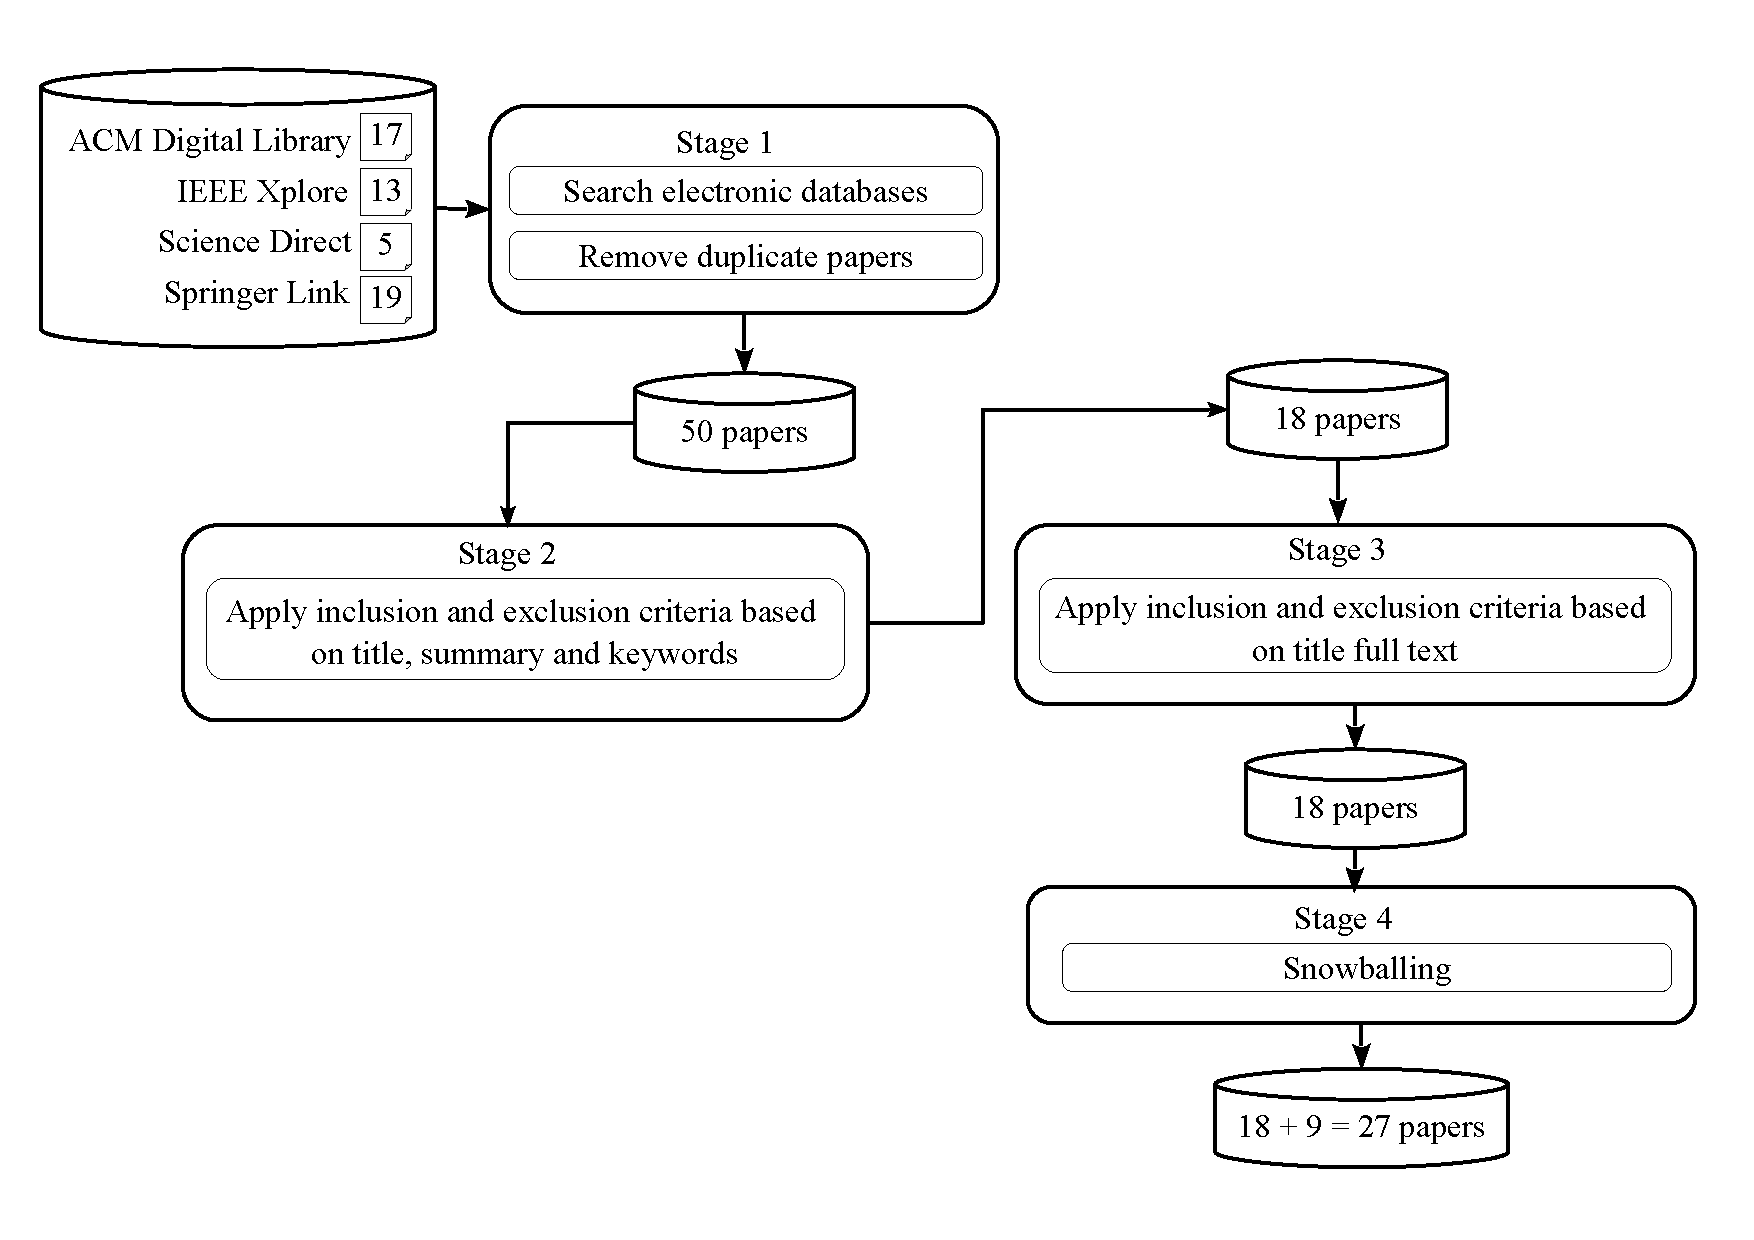
\includegraphics[width=.9\textwidth]{figures/smr-selection-phases.pdf}
  \caption{Diagram of the four-stage paper selection process.}
  \label{fig:smr_selection_phases}
\end{figure}

\begin{table*}[h!]
  \centering
  \spacebtrows{1.3}
  \caption{Selected papers}
  \begin{tabular}{@{}lp{18cm}@{}} 
    \toprule
    ID & Bibliographic reference\\ 
    \midrule
    %  \#1 & A. Lamkanfi, S. Demeyer, E. Giger and B. Goethals, ``Predicting the severity of a reported bug," 2010 7th IEEE Working Conference on Mining Software Repositories (MSR 2010), Cape Town, 2010, pp. 1-10.\\
    \cite{Lamkanfi:2010} & \vspace{-0.2cm}\bibentry{Lamkanfi:2010}. doi:\href{https://doi.org/10.1109/MSR.2010.5463284}{10.1109/MSR.2010.5463284}.\\
    
    %  \#2 & A. Lamkanfi, S. Demeyer, Q. D. Soetens and T. Verdonck, ``Comparing Mining Algorithms for Predicting the Severity of a Reported Bug", 2011 15th European Conference on Software Maintenance and Reengineering, Oldenburg, 2011, pp. 249-258.\\
    \cite{Lamkanfi:2011} & \vspace{-0.2cm}\bibentry{Lamkanfi:2011}. doi:\href{https://doi.org/10.1109/CSMR.2011.31}{10.1109/CSMR.2011.31}.\\
    
    %  \#3 & Y. Tian, D. Lo and C. Sun, ``Information Retrieval Based Nearest Neighbor Classification for Fine-Grained Bug Severity Prediction," 2012 19th Working Conference on Reverse Engineering, Kingston, ON, 2012, pp. 215-224.\\ 
    \cite{Tian:2012} & \vspace{-0.2cm}\bibentry{Tian:2012}.  doi:\href{https://doi.org/10.1109/WCRE.2012.31}{10.1109/WCRE.2012.31}.\\
    
    %  \#4 & C. Z. Yang, C. C. Hou, W. C. Kao and I. X. Chen, ``An Empirical Study on Improving Severity Prediction of Defect Reports Using Feature Selection," 2012 19th Asia-Pacific Software Engineering Conference, Hong Kong, 2012, pp. 240-249.\\
    \cite{Yang:2012} & \vspace{-0.2cm}\bibentry{Yang:2012}.  doi:\href{https://doi.org/10.1109/APSEC.2012.144}{10.1109/APSEC.2012.144}.\\
    
    %  \#5 & Chaturvedi, K. K. and V.B. Singh. ``An Empirical Comparison of Machine Learning Techniques in Predicting the Bug Severity of Open and Closed Source Projects." IJOSSP 4.2 (2012): 32-59. \\ 
    \cite{Chaturvedi:2012} & \vspace{-0.2cm}\bibentry{Chaturvedi:2012}.  doi:\href{https://doi.org/10.4018/jossp.2012040103}{10.4018/jossp.2012040103}.\\
    
    %  \#6 & C. Z. Yang, K. Y. Chen, W. C. Kao and C. C. Yang, ``Improving severity prediction on software bug reports using quality indicators," 2014 IEEE 5th International Conference on Software Engineering and Service Science, Beijing, 2014, pp. 216-219.\\ 
    \cite{Yang:2014a} & \vspace{-0.2cm}\bibentry{Yang:2014a}.  doi:\href{https://doi.org/10.1109/ICSESS.2014.6933548}{10.1109/ICSESS.2014.6933548}.\\ 
    
    %  \#7 & G. Yang, T. Zhang and B. Lee, ``Towards Semi-automatic Bug Triage and Severity Prediction Based on Topic Model and Multi-feature of Bug Reports," 2014 IEEE 38th Annual Computer Software and Applications Conference, Vasteras, 2014, pp. 97-106.\\ 
    \cite{Yang:2014b} & \vspace{-0.2cm}\bibentry{Yang:2014b}.  doi:\href{https://doi.org/10.1109/COMPSAC.2014.16}{10.1109/COMPSAC.2014.16}.\\
    
    %  \#8 & Harold Valdivia Garcia and Emad Shihab. 2014. ``Characterizing and predicting blocking bugs in open source projects". In Proceedings of the 11th Working Conference on Mining Software Repositories (MSR 2014). ACM, New York, NY, USA, 72-81.\\
    \cite{Valdivia:2014} & \vspace{-0.2cm}\bibentry{Valdivia:2014}.  doi:\href{https://doi.org/10.1145/2597073.2597099}{10.1145/2597073.2597099}\\
    
    %  \#9 & Sharma M., Kumari M., Singh R.K., Singh V.B. (2014) ``Multiattribute Based Machine Learning Models for Severity Prediction in Cross Project Context". In: Murgante B. et al. (eds) Computational Science and Its Applications – ICCSA 2014. ICCSA 2014. Lecture Notes in Computer Science, vol 8583. Springer, Cham.\\ 
    \cite{Meera:2014} & \vspace{-0.2cm}\bibentry{Meera:2014}.  doi:\href{https://doi.org/10.1007/978-3-319-09156-3\_17}{10.1007/978-3-319-09156-3\_17}\\
    
    %  \#10 & N. K. S. Roy and B. Rossi, ``Towards an Improvement of Bug Severity Classification," 2014 40th EUROMICRO Conference on Software Engineering and Advanced Applications, Verona, 2014, pp. 269-276.\\ 
    \cite{Roy:2014} & \vspace{-0.2cm}\bibentry{Roy:2014}.  doi:\href{https://doi.org/10.1109/SEAA.2014.51}{10.1109/SEAA.2014.51}\\
    
    %  \#11 & Ripon K. Saha, Julia Lawall, Sarfraz Khurshid, and Dewayne E. Perry. 2015. ``Are these bugs really ``normal"?''. In Proceedings of the 12th Working Conference on Mining Software Repositories (MSR '15). IEEE Press, Piscataway, NJ, USA, 258-268.\\ 
    \cite{Saha:2015} & \vspace{-0.2cm}\bibentry{Saha:2015}.  doi:\href{https://doi.org/10.1109/MSR.2015.31}{10.1109/MSR.2015.31}\\
    
    %  \#12 & Tao Zhang, Geunseok Yang, Byungjeong Lee, and Alvin T. S. Chan. 2015. ``Predicting severity of bug report by mining bug repository with concept profile". In Proceedings of the 30th Annual ACM Symposium on Applied Computing (SAC '15). ACM, New York, NY, USA, 1553-1558.\\ 
    \cite{Zhang:2015} & \vspace{-0.2cm}\bibentry{Zhang:2015}.  doi:\href{https://doi.org/10.1145/2695664.2695872}{10.1145/2695664.2695872}\\
    
    %  \#13 & G. Sharma, S. Sharma, S. Gujral, ``A Novel Way of Assessing Software Bug Severity Using Dictionary of Critical Terms", Procedia Computer Science, pp. 632-639, 2015.\\ 
    \cite{Sharma:2015} & \vspace{-0.2cm}\bibentry{Sharma:2015}.  doi:\href{https://doi.org/10.1016/j.procs.2015.10.059}{10.1016/j.procs.2015.10.059}\\
    
    %  \#14 & X. Xia, D. Lo, E. Shihab, X. Wang, X. Yang, ``Elblocker: Predicting blocking bugs with ensemble imbalance learning", Information and Software Technology, 2015.\\ 
    \cite{Xia:2015} & \vspace{-0.2cm}\bibentry{Xia:2015}.  doi:\href{https://doi.org/10.1016/j.infsof.2014.12.006}{10.1016/j.infsof.2014.12.006}\\
    
    %  \#15 & S. Gujral, G. Sharma, S. Sharma and Diksha, ``Classifying bug severity using dictionary-based approach," 2015 International Conference on Futuristic Trends on Computational Analysis and Knowledge Management (ABLAZE), Noida, 2015, pp. 599-602.\\ 
    \cite{Gujral:2015} & \vspace{-0.2cm}\bibentry{Gujral:2015}.  doi:\href{https://doi.org/10.1109/ABLAZE.2015.7154933}{10.1109/ABLAZE.2015.7154933}\\
    
    %  \#16 & M. N. Pushpalatha and M. Mrunalini, ``Predicting the severity of bug reports using classification algorithms," 2016 International Conference on Circuits, Controls, Communications and Computing (I4C), Bangalore, 2016, pp. 1-4.\\ 
    \cite{Pushpalathas:2016} & \vspace{-0.2cm}\bibentry{Pushpalathas:2016}.  doi:\href{https://doi.org/10.1109/CIMCA.2016.8053276}{10.1109/CIMCA.2016.8053276}\\
    
    %  \#17 & A. F. Otoom, D. Al-Shdaifat, M. Hammad and E. E. Abdallah, ``Severity prediction of software bugs," 2016 7th International Conference on Information and Communication Systems (ICICS), Irbid, 2016, pp. 92-95.\\ 
    \cite{Otoom:2016} & \vspace{-0.2cm}\bibentry{Otoom:2016}.  doi:\href{https://doi.org/10.1109/IACS.2016.7476092}{10.1109/IACS.2016.7476092}\\  
    
    % \#18 & Korosh Koochekian Sabor, Mohammad Hamdaqa, and Abdelwahab Hamou-Lhadj. 2016. ``Automatic prediction of the severity of bugs using stack traces". In Proceedings of the 26th Annual International Conference on Computer Science and Software Engineering (CASCON '16), Blake Jones (Ed.). IBM Corp., Riverton, NJ, USA, 96-105. \\ 
    \cite{Sabor:2016} & \vspace{-0.2cm}\bibentry{Sabor:2016}.\\  
    
    %  \#19 & Tian, Y., Ali, N., Lo, D. et al. Empir Software Eng (2016) 21: 2298. https://doi.org/10.1007/s10664-015-9409-1\\ 
    \cite{Tian:2016} & \vspace{-0.2cm}\bibentry{Tian:2016}.  doi:\href{https://doi.org/10.1007/s10664-015-9409-1}{10.1007/s10664-015-9409-1}\\
    
    %  \#20 & Tao Zhang, Jiachi Chen, Geunseok Yang, Byungjeong Lee, and Xiapu Luo. 2016. ``Towards more accurate severity prediction and fixer recommendation of software bugs". J. Syst. Softw. 117, C (July 2016), 166-184. \\ 
    \cite{Zhang:2016} & \vspace{-0.2cm}\bibentry{Zhang:2016}.  doi:\href{https://doi.org/10.1016/j.jss.2016.02.034}{10.1016/j.jss.2016.02.034}\\
    
    %  \#21 & Kwanghue, J., Amarmend, D., Geunseok, Y., Jung-Won, L., Byungjeong, L.: ``Bug severity prediction by classifying normal bugs with text and meta-field information". Adv. Sci. Technol. Lett. 129 (2016). Mechanical Engineering.\\ 
    \cite{Jin:2016a} & \vspace{-0.2cm}\bibentry{Jin:2016a}.  doi:\href{http://dx.doi.org/10.14257/astl.2016.129.05}{10.14257/astl.2016.129.05}\\
    
    %  \#22 & T. Choeikiwong, P. Vateekul, ``Improve accuracy of defect severity categorization using semi-supervised approach on imbalanced data sets", Proceedings of the International MultiConference of Engineers and Computer Scientists, vol. 1, 2016.\\ 
    \cite{Choeikiwong:2016} & \vspace{-0.2cm}\bibentry{Choeikiwong:2016}.\\
    
    %  \#23 & Jin, Kwanghue, Dashbalbar, Amarmend Yang, Geunseok, Lee, Byungjeong, Lee, Jung-Won. (2016). ``Improving predictions about bug severity by utilizing bugs classified as normal". Contemporary Engineering Sciences. 9. 933-942. 10.12988/ces.2016.6695.\\ 
    \cite{Jin:2016b} & \vspace{-0.2cm}\bibentry{Jin:2016b}.  doi:\href{http://dx.doi.org/10.12988/ces.2016.6695}{10.12988/ces.2016.6695}\\
    
    %  \#24 & Jin, K, Lee, E.C., Dashbalbar, A, Lee, J, Lee, B. (2016). ``Utilizing feature based classification and textual information of bug reports for severity prediction". 19. 651-659. \\
    \cite{Jin:2016c} & \vspace{-0.2cm}\bibentry{Jin:2016c}.\\
    
    %  \#25 & Geunseok Yang, Seungsuk Baek, Jung-Won Lee, and Byungjeong Lee. 2017. ``Analyzing emotion words to predict severity of software bugs: a case study of open source projects". In Proceedings of the Symposium on Applied Computing (SAC '17). ACM, New York, NY, USA, 1280-1287. \\ 
    \cite{Yang:2017} & \vspace{-0.2cm}\bibentry{Yang:2017}.  doi:\href{http://doi.org/10.1145/3019612.3019788}{10.1145/3019612.3019788}\\
    
    %  \#26 & V. B. Singh, Sanjay Misra, and Meera Sharma, J. Info. Know. Mgmt. 16, 1750005 (2017)\\ 
    \cite{Singh:2017} & \vspace{-0.2cm}\bibentry{Singh:2017}.  doi:\href{http://doi.org/10.1142/S0219649217500058}{10.1142/S0219649217500058}\\
    
    %  \#27 & N. K. S. Roy and B. Rossi, ``Cost-Sensitive Strategies for Data Imbalance in Bug Severity Classification: Experimental Results," 2017 43rd Euromicro Conference on Software Engineering and Advanced Applications (SEAA), Vienna, 2017, pp. 426-429.\\     
    \cite{Roy:2017} & \vspace{-0.2cm}\bibentry{Roy:2017}.  doi:\href{http://doi.org/10.1109/SEAA.2017.71}{10.1109/SEAA.2017.71}\\
    
    \bottomrule
  \end{tabular}
  \label{tab:selected_studies}
\end{table*}

\subsection{Limitations of this mapping}\label{subsec:limitations}
To interpret the implications of our results adequately, one needs to consider the following common limitations of all mapping reviews:
\begin{itemize}
  \item \textbf{Mapping review completeness can never be guaranteed~\cite{Brhel:2015}}: Although this mapping review has observed a strict research protocol to ensure the relatively whole population of the relevant literature, some important papers might be missed.
  \item \textbf{Terminology problems in search string may lead to miss some primary studies~\cite{Desouza:2015}}: The terminology applied in the database query is normally accepted and used within the scientific community. Nevertheless, different terms may be used to retrieve the same relevant information.
  \item \textbf{Subjective evaluation of inclusion and exclusion criteria may cause misinterpretation~\cite{Brhel:2015}}. Explicit criteria have been defined for assessing the relevance of selected papers~\ref{subsec:selection}. However, the evaluation was based on the perception and experience of the authors. Different people may have other views regarding the relevance of these papers.
\end{itemize}

\subsection{Categorization scheme}\label{subsec:categorization}
Petersen et al.\cite{Petersen:2008} suggest the definition of a categorization scheme for conducting a systematic mapping analysis. The categories defined for this mapping review were based on: (i) existing labels commonly used in the literature and (ii) the content of selected papers. Next sections outline the categories considered in this mapping review.

\subsubsection{FLOSS software type~($RQ_{2}$)}
This scheme organizes FLOSS projects by software type. Based on the taxonomy suggested by Pressman~\cite{Pressman:2009}, FLOSS in studies belongs to three categories: 

\begin{enumerate}[label=\alph*., leftmargin=1.2cm]
  \item \textbf{Application software}: This category includes computer programs designed to solve a specific problem or business need for end users. 
  \item \textbf{System software}: This category includes collections of computer programs (operating systems and utilities) required to run and maintain a computer system.
  \item \textbf{Programming tools}: This category includes computer programs that aid software developers in creating, debugging, maintain or perform any development-specific task.
\end{enumerate}

\subsubsection{Severity prediction problem~($RQ_{3}$)}
This scheme drills down severity prediction problems, based on studying of selected papers, in five categories:

\begin{enumerate}[label=\alph*., leftmargin=1.2cm]
  \item \textbf{Severe or Non-Severe (SNS)}: This category comprises the prediction problems whose the predicted severity level might be severe or non-severe. In Bugzilla, for example, the severe class would include blocker, critical, and major; and the non-severe class would include minor and trivial levels. The predictors of this problem category do not take into account the default severity level.
  
  \item \textbf{Severe or Non-Severe With Default Class (SNSWD)}: This category is quite similar to SNS. However, the predictors consider the default severity level as severe or non-severe, or yet as another class.
  
  \item \textbf{Multiple Classes (MC)}: This category comprises prediction problems whose predictors treat each severity level as a different class. Likewise that in SNS, the predictors do not take into account the default severity level.
  
  \item \textbf{Multiple Classes With Default Class (MCWD)}: This category is similar to MC. However, the predictors consider the default severity level as a regular class.
  \item \textbf{Blocking or Non-Blocking (BNB)}: The prediction problem whose predictors classify a bug report severity level into blocking or non-blocking class. A blocking bug is a software defect that prevents other defects from being fixed\cite{Valdivia:2014}. 
\end{enumerate}


\subsubsection{Feature data types~($RQ_4$)}
This scheme groups the features used for bug reports severity prediction into five categories: 

\begin{enumerate}[label=\alph*., leftmargin=1.2cm]
  \item \textbf{Qualitative categorical}: This category encompasses features that contain an unordered list of values. For instance, 
  bug report \textit{platform} attribute (e.g., ``Windows", ``Linux", ``Android"). 
  \item \textbf{Qualitative ordinal}: This category encompasses features that contain an ordered list of values. For instance, bug report \textit{priority} attribute (e.g., P1, P2, P3). 
  \item \textbf{Quantitative discrete}: This category encompasses features that contain a finite or an infinite number of values that can be counted, such as the \textit{bug fixed time} attribute. 
  \item \textbf{Quantitative continuous}: This category encompasses features that contain an infinite number of values that can be measured, such as the \textit{summary weight} attribute.
  \item \textbf{Unstructured text}: This category encompasses features that either do not have a pre-defined data model or are not organized in a pre-defined manner. For instance, the bug report \textit{description} attribute usually includes free format texts.
\end{enumerate}

\subsubsection{Feature selection methods~($RQ_5$)}
This scheme organizes the feature selection methods used for bug reports severity prediction into three categories, according to the taxonomy described in Guyon and Elisseeff~\cite{Guyon:2003}:

\begin{enumerate}[label=\alph*., leftmargin=1.2cm]
  \item \textbf{Filter}: This category comprises methods that assign a score to the features, and use this value as a selection criterion to identify the top-scoring ones.
  \item \textbf{Wrapper}: This category comprises methods that prepare, evaluate and compare feature combinations, and select the best one. Methods within this category consider the feature selection as a search problem.
  \item \textbf{Embedded}: This category comprises methods that select which features best contribute to the accuracy while the ML algorithm creates the predicting model.
\end{enumerate}

\subsubsection{Text mining feature representations~($RQ_6$)}
This scheme organizes the techniques for text mining feature representations used for bug report severity prediction in four categories. The following categories were employed in this systematic mapping review according to \cite{Feldman:2006}:

\begin{enumerate}[label=\alph*., leftmargin=1.2cm]
  \item \textbf{Character}: This category includes techniques that represent features as individual component-level letters, numerals, special characters, and spaces are the building blocks of higher-level semantic features, such as words, terms, and concepts.
  \item \textbf{Word}: This category includes techniques that represent features as specific words selected directly from a ``native" document.
  \item \textbf{Term}: This category includes techniques that represent features as single words and multiword phrases selected directly from a corpus of a native document using a term-extraction method. 
  \item \textbf{Concept}: This category includes techniques that represent features generated for a document employing manual, statistical, rule-based, or hybrid categorization methodologies.
\end{enumerate}

\subsubsection{ML algorithms categories ($RQ_7$)}
This scheme groups ML algorithms used in bug report severity prediction in five categories. The following categories were based on taxonomy proposed by Facelli et al.~\cite{Facelli:2015}:

\begin{enumerate}[label=\alph*., leftmargin=1.2cm]
  \item \textbf{Distance-based}: This category comprises algorithms that use the proximity between data to generate their predictions.
  \item \textbf{Probabilistic-based}: This category comprises algorithms that make their predictions based on the Bayes's theorem.
  \item \textbf{Searching-based}: This category comprises algorithms that rely on searching for a solution in space to generate their predictions.
  \item \textbf{Optimization-based}: This category comprises algorithms whose predictions are based on an optimization function.
  \item \textbf{Ensemble-method}: This category comprises algorithms that combine or aggregate results of different base classifiers to make a prediction.
\end{enumerate}

\subsubsection{Evaluation measures categories ($RQ_8$)}
This scheme organizes evaluation measures used in selected papers by categories. According to Japkowicz and Shah~\cite{Japkowicz:2011},
there are six categories:  

\begin{enumerate}[label=\alph*., leftmargin=1.2cm]
  \item \textbf{Single class focus}: This category comprises measures based on confusion matrix information, whose focus is on a single class of interest.
  \item \textbf{Multi-class focus}: This category comprises measures based on confusion matrix information, whose focus is on all the classes of the problem domain.
  \item \textbf{Graphical measure}: This category comprises measures based on a confusion matrix in conjunction with extra information. They enable visualization of the classifier performance under different skew ratios and class priors distribution and are indicated for scoring classifiers.
  \item \textbf{Summary statistics}: This category comprises measures based on a confusion matrix in conjunction with extra information. They enable to quantify the comparative analysis between classifiers and are indicated for scoring classifiers.
  \item \textbf{Distance/error-measure}: This category comprises measures based on a confusion matrix in conjunction with extra information. They measure the distance of an instance's predicted class label to its actual label and are recommended for continuous and probabilistic classifiers.
  \item \textbf{Information theoretic measures}: This category comprises measures based on a confusion matrix in conjunction with extra information. They reward a classifier upon correct classification relative to the (typically empirical) prior to the data and are indicated for continuous and probabilistic classifiers.
\end{enumerate}

\subsubsection{Sampling techniques ($RQ_9$)}
This scheme organizes the sampling techniques used for bug report severity prediction into three categories. Such categories according to Japkowicz and Shah~\cite{Japkowicz:2011} include:

\begin{enumerate}[label=\alph*., leftmargin=1.2cm]
  \item \textbf{No re-sampling}: This category encompasses techniques that test the algorithm on a large set of unseen data.
  \item \textbf{Simple re-sampling}: This category encompasses techniques that use each data point for testing only once. 
  \item \textbf{Multiple re-sampling}: This category encompasses techniques that use each data point for testing more than once. 
\end{enumerate}

\subsubsection{Statistical Tests ($RQ_{10}$)}
This scheme groups statistical tests commonly used for bug report severity prediction in three categories. Such categories employed in this mapping review according to Japkowicz and Shah~\cite{Japkowicz:2011} include:

\begin{enumerate}[label=\alph*., leftmargin=1.2cm]
  \item \textbf{Parametric}: This category comprises methods that make strong assumptions about the distribution of the population
  \item \textbf{Non-parametric}: This category comprises methods that do not make strong assumptions about the distribution of the population
  \item \textbf{Parametric and non-parametric}: This category comprises methods that are both parametric and non-parametric
\end{enumerate}

\subsubsection{Experiment software tools ($RQ_{11}$)}
This scheme groups the software tools used in experiments for bug reports severity prediction in two well-known and popular categories: 

\begin{enumerate}[label=\alph*., leftmargin=1.2cm]
  \item \textbf{Free/Libre Open Source Software (FLOSS)}: This category includes software that can be freely used, modified, and redistributed.
  \item \textbf{Closed Source Software (CSS)}: This category includes software that is owned by an individual or a company whose source code is not shared with the public for anyone to look at or change. 
\end{enumerate}
\section{Results}  \label{sec:results}
This section summarizes the results of this mapping review. The answer to each research question (from RQ1 to RQ12) is presented in tables and charts. The organization of extracted data follows the criteria defined in Section~\ref{sec:research_method}. 

\subsection{When and where have the studies been published? (RQ1)}\label{subsec:rq1}

Figure~\ref{fig:classification_by_publication_year} shows that research on bug report severity prediction in FLOSS is recent and active with a vast number of papers (22 out of 27 $\approx$ 81\%) published from 2014. Journals and conferences on information technology, mining software repositories, and software engineering seem to be more open to papers of bug report severity prediction (Table \ref{tab:papers_sources}). 

\begin{table}[h!]
  \centering
  \caption{Papers publication sources.}
  \begin{tabular}{@{}llr@{}} 
    \toprule
    \textbf{Paper source} & \textbf{Type} & \textbf{Reference} \\ 
    \midrule
    ACM Symposium on Applied Computing                 & Conference     & \cite{Zhang:2015}\\ 
    \midrule
    Advanced Science and Technology Letters \& Journal & Journal         & \cite{Jin:2016a}\\
    \midrule
    Asia-Pacific Software Engineering Conference         & Conference     & \cite{Yang:2012}\\
    \midrule
    Computational Science and Its Applications (ICCSA)     & Conference     & \cite{Meera:2014}\\
    \midrule
    Computer Software and Applications Conference         & Conference     & \cite{Yang:2014b}\\
    \midrule
    Contemporary Engineering Sciences                     & Journal         & \cite{Jin:2016b}\\
    \midrule
    Empirical Software Engineering                     & Journal         & \cite{Tian:2016}\\
    \midrule
    Futuristic Trends on Computational Analysis and Knowledge Management (ABLAZE) & Conference & \cite{Gujral:2015}\\
    \midrule
    Information and Software Technology                 & Journal         & \cite{Xia:2015}\\
    \midrule
    International Conference on Circuits, Controls, Communications and Computing (I4C) & Conference & \cite{Pushpalathas:2016}\\
    \midrule
    International Conference on Computer Science and Software Engineering         & Conference & \cite{Sabor:2016}\\
    \midrule
    International Conference on Information and Communication Systems (ICICS)     & Conference & \cite{Otoom:2016}\\
    \midrule
    International Conference on Software Engineering and Service Science        & Conference & \cite{Yang:2014a}\\
    \midrule
    International Information Institute                                 & Journal         & \cite{Jin:2016c}\\
    \midrule
    International Journal of Open Source Software and Process(IJOSSP)    & Journal         & \cite{Chaturvedi:2012}\\
    \midrule
    International MultiConference of Engineers and Computer Scientists     & Conference     & \cite{Choeikiwong:2016}\\
    \midrule
    Journal of Information \& Knowledge Management                         & Journal         & \cite{Singh:2017}\\
    \midrule
    Journal of Systems and Software                 & Journal     & \cite{Zhang:2016}\\
    \midrule
    Procedia Computer Science                     & Journal     & \cite{Sharma:2015}\\
    \midrule
    Software Engineering and Advanced Applications (SEAA) & Conference & \cite{Roy:2014}, \cite{Roy:2017}\\
    \midrule
    Symposium on Applied Computing (SAC)         & Conference & \cite{Yang:2017}\\
    \midrule
    Working Conference on Mining Software Repositories (MSR) & Conference & \cite{Lamkanfi:2010}, \cite{Lamkanfi:2011}, \cite{Valdivia:2014}, \cite{Saha:2015}\\
    \midrule
    Working Conference on Reverse Engineering     & Conference & \cite{Tian:2012} \\
    \bottomrule
  \end{tabular}
  \label{tab:papers_sources}
\end{table}

\subsection{What FLOSS are the most used as experimental target for bug report severity prediction (RQ2)?}\label{subsec:rq2_result}

Table \ref{tab:papers_by_floss} shows that most papers concentrated their focus on five FLOSS: Eclipse ($\approx$ 92\%), Mozilla ($\approx$ 70\%), Openoffice ($\approx$ 18\%), Netbeans ($\approx$ 14\%), and Gnome ($\approx$ 11\%). The detailing of each FLOSS including description, category, BTS, and URL is presented in Table \ref{tab:floss_descriptions}.

\begin{table}[h!]
  \vspace{0pt}
  \centering
  \captionsetup{type=table}
  \caption{Paper distribution by FLOSS.}
  \small
  \begin{tabular}{@{}lp{10cm}r@{}}
    \toprule
    \textbf{Project} & \textbf{References} & \textbf{Total}\\
    \midrule
    Eclipse & \cite{Lamkanfi:2010},\cite{Lamkanfi:2011},\cite{Tian:2012},\cite{Yang:2012},\cite{Chaturvedi:2012},\cite{Yang:2014b},\cite{Yang:2014a},\cite{Valdivia:2014},\cite{Roy:2014},\cite{Saha:2015},\cite{Zhang:2015},\cite{Sharma:2015},\cite{Xia:2015},\cite{Gujral:2015},\cite{Otoom:2016},\cite{Sabor:2016},\cite{Tian:2016},\cite{Zhang:2016},\cite{Jin:2016a},\cite{Choeikiwong:2016},\cite{Jin:2016b},\cite{Jin:2016c},\cite{Yang:2017},\cite{Singh:2017},\cite{Roy:2017},\cite{Lamkanfi:2011},\cite{Tian:2012},\cite{Yang:2012},\cite{Chaturvedi:2012},\cite{Yang:2014b},\cite{Yang:2014a},\cite{Valdivia:2014},\cite{Roy:2014},\cite{Saha:2015},\cite{Zhang:2015},\cite{Sharma:2015},\cite{Xia:2015},\cite{Gujral:2015},\cite{Otoom:2016},\cite{Sabor:2016},\cite{Tian:2016},\cite{Zhang:2016},\cite{Jin:2016a},\cite{Choeikiwong:2016},\cite{Jin:2016b},\cite{Jin:2016c},\cite{Yang:2017},\cite{Singh:2017},\cite{Roy:2017} & 25 \\
    \midrule
    Mozilla & \cite{Lamkanfi:2010},\cite{Tian:2012},\cite{Yang:2012},\cite{Chaturvedi:2012},\cite{Yang:2014b},\cite{Valdivia:2014},\cite{Meera:2014},\cite{Roy:2014},\cite{Zhang:2015},\cite{Xia:2015},\cite{Pushpalathas:2016},\cite{Otoom:2016},\cite{Tian:2016},\cite{Zhang:2016},\cite{Jin:2016a},\cite{Jin:2016b},\cite{Jin:2016c},\cite{Singh:2017},\cite{Roy:2017} & 19 \\
    \midrule
    Openoffice & \cite{Tian:2012},\cite{Valdivia:2014},\cite{Xia:2015},\cite{Tian:2016},\cite{Zhang:2016} & 5 \\
    \midrule
    Netbeans & \cite{Yang:2014b},\cite{Valdivia:2014},\cite{Xia:2015},\cite{Zhang:2016} & 4 \\
    \midrule
    Gnome & \cite{Lamkanfi:2010},\cite{Lamkanfi:2011},\cite{Chaturvedi:2012} & 3 \\
    \midrule
    Chromium & \cite{Valdivia:2014},\cite{Xia:2015} & 2 \\
    Freedesktop & \cite{Valdivia:2014},\cite{Xia:2015} & 2 \\
    \midrule
    GCC & \cite{Zhang:2016} & 1 \\
    \midrule
    Hibernate & \cite{Roy:2017} & 1 \\
    \midrule
    Spring & \cite{Roy:2017} & 1 \\
    \midrule
    Android & \cite{Yang:2017} & 1 \\
    \midrule
    JBoss & \cite{Yang:2017} & 1 \\
    \midrule
    Mongo-db & \cite{Roy:2017} & 1 \\
    \midrule
    WineHQ & \cite{Pushpalathas:2016} & 1 \\
    \bottomrule
  \end{tabular} 
  \label{tab:papers_by_floss}  
\end{table} 

Figure \ref{fig:distribution_by_floss} shows that most papers worked with FLOSS  related to Programming Tool ($\approx$ 92\%) and Application Software ($\approx$  74\%) categories. Moreover, it presents that 17 out of 27 ($\approx$ 62\%) papers worked with both categories. Figure \ref{fig:distribution_by_bts} highlights that all papers handled bug reports extracted from Bugzilla, and a just few papers from Google (3 out of 27 - $\approx$ 11\%) and Jira (2 out of 27 $\approx$ 7\%). Only one paper (Yang et al.\cite{Yang:2017}) investigated bug reports from three BTS.

\begin{table*}[h!]
  \centering
  \caption{FLOSS investigated in papers.}
  \begin{tabular}{@{}lllll@{}} 
    \toprule
    \textbf{Project} & \textbf{Description} & \textbf{Category} & \textbf{BTS} & \textbf{URL (As of \today)}\\ 
    \midrule
    Android        &  Mobile operating system     & System software & Google       & \url{https://issuetracker.google.com}            \\ 
    Chromium    &  Web browser                 & Application software & Google       & \url{https://www.chromium.org/issue-tracking}    \\ 
    Eclipse        &  Integrated Development Environment(IDE) &  Programming tool & Bugzilla  & \url{https://bugs.eclipse.org/bugs/}            \\ 
    FreeDesktop &  Base platform for desktop software on Linux and UNIX & Programing Tool & Bugzilla  & \url{https://bugs.freedesktop.org/}            \\ 
    GCC            &  C compiler                 & Programming tool & Bugzilla  & \url{https://gcc.gnu.org/bugzilla/}            \\ 
    Gnome        &  Desktop environment based on X Windows System & Application Software & Bugzilla  & \url{https://gcc.gnu.org/bugzilla/}            \\ 
    Hibernate    &  Object Relation Mapper(ORM) framework & Programming tool & Jira      & \url{https://hibernate.atlassian.net}            \\ 
    Jboss        &  Application server         & System software & Jira       & \url{https://issues.jboss.org/s}                \\ 
    Mongo-db    &  No-sql database             & System software & Jira       & \url{https://jira.mongodb.org/}                \\ 
    Mozilla        &  Internet tools             & Application software & Bugzilla     & \url{https://bugzilla.mozilla.org/}            \\ 
    Netbeans    &  Integrated Development Environment(IDE) & Programming tool    & Bugzilla  & \url{https://netbeans.org/bugzilla/}            \\ 
    OpenOffice    &  Office suite             & Application software & Bugzilla    & \url{https://bz.apache.org/ooo/}                \\ 
    Spring        &  JEE Framework             & Programming tool & Jira       & \url{https://jira.spring.io}                    \\ 
    WineHQ        &  Compatibility layer         & System software & Bugzilla  & \url{https://bugs.winehq.org/}                \\ 
    \bottomrule
  \end{tabular}
  \label{tab:floss_descriptions}
\end{table*}

%%%%
\begin{figure}[!htp]
  \begin{subfigure}{.94\textwidth}
    \centering
    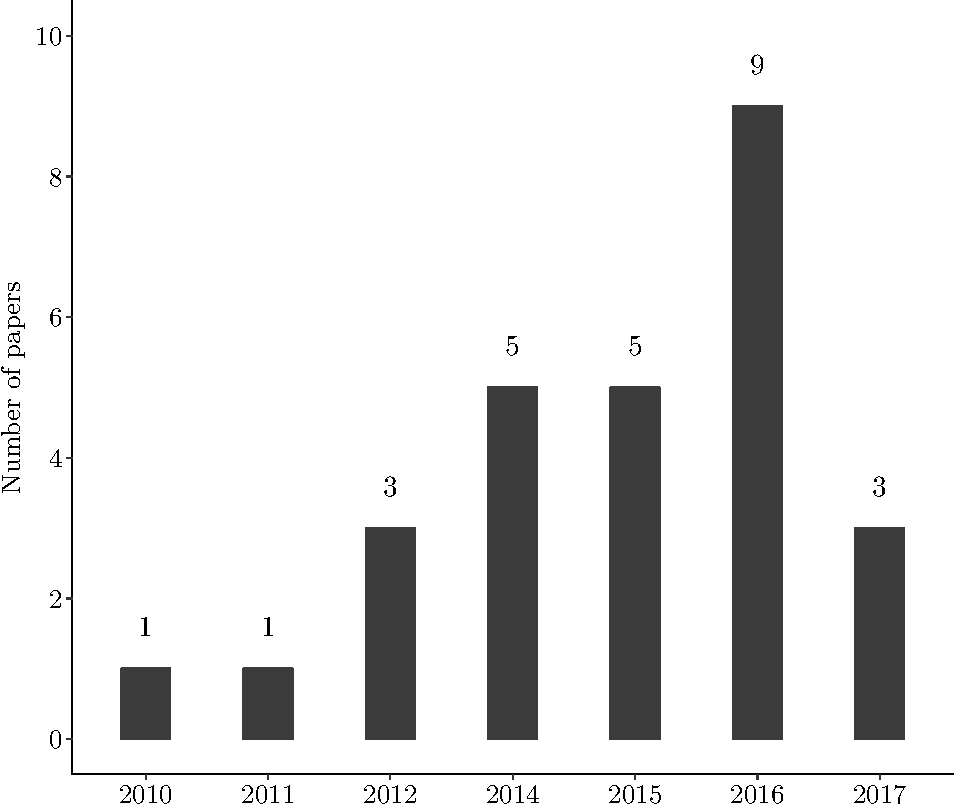
\includegraphics[width=0.5\textwidth]{figures/survey-summary-by-year-in-bar.pdf}
    \caption{}    
    \label{fig:classification_by_publication_year}
  \end{subfigure}\hfill
  %  \begin{subfigure}{.30\textwidth}
  %    \centering
  %    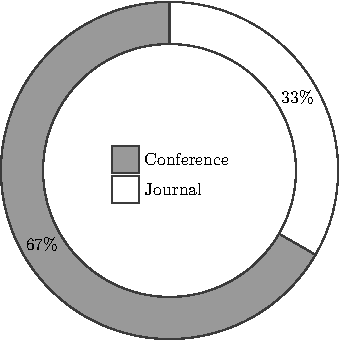
\includegraphics[width=0.9\textwidth]{figures/survey-summary-by-source-in-dnt.pdf}
  %    \caption{}
  %    \label{fig:classification_by_publication_source} 
  %  \end{subfigure}\hfill
  \begin{subfigure}{.49\textwidth}
    \centering
    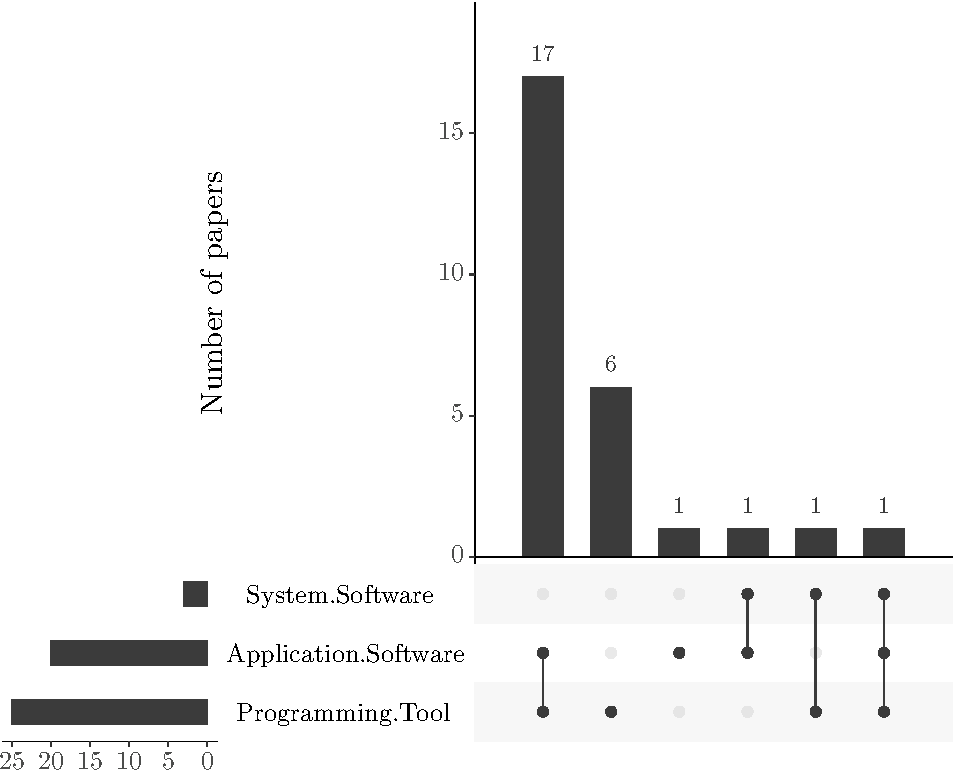
\includegraphics[width=\textwidth]{figures/distribution-by-floss-in-ups.pdf}
    \caption{}
    \label{fig:distribution_by_floss}
  \end{subfigure}\hfill
  \begin{subfigure}{.49\textwidth}
    \centering
    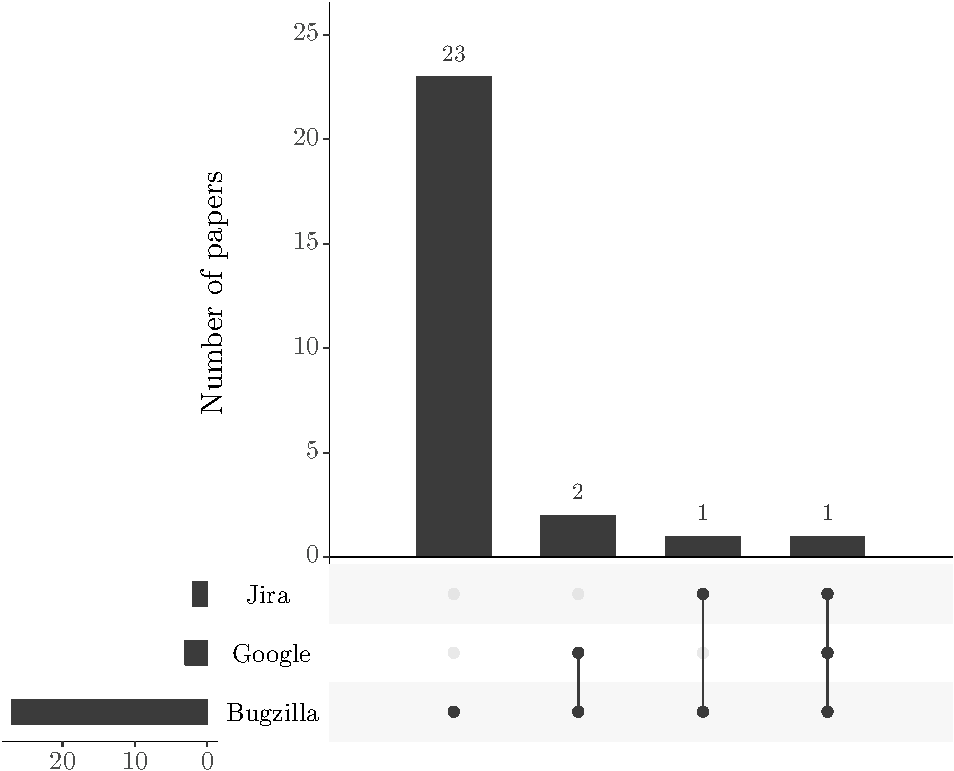
\includegraphics[width=\textwidth]{figures/distribution-by-bts-in-ups.pdf}
    \caption{}
    \label{fig:distribution_by_bts} 
  \end{subfigure}
  \caption{(a) Paper distribution by year (67\% published in conferences and 33\% in journals), (b) paper distribution by FLOSS (c) paper distribution by BTS.}
  \label{fig:rq1_classification}
\end{figure}
%%%%

\subsection{Was bug report severity prediction most addressed as either a fine-grained label  or coarse-grained label prediction problem (RQ3)?}\label{subsec:rq3_result}

Table~\ref{tab:prediction_problem_type_by_paper} shows that about the same fraction of papers addressed the bug report severity prediction as coarse-grained and fine-grained problem. Figure \ref{fig:distribution_by_problem-category_in_ups} shows that most papers  (10 out of 27 $\approx$ 37\%)  addressed the severity prediction as a problem of SNS category. Moreover, 8 out of 27 ($\approx$ 20\%) papers addressed it as a problem of the MC category and 5 out of 27 ($\approx$ 18.5\%) addressed a problem of the MCWD category. A few papers addressed a BNB (2 out of 27 $\approx$ 7\%) or an SNSWD (2 out of 27 $\approx$ 7\%) problem. No paper addressed more than one problem category.

\begin{table*}[h!]
  \vspace{30pt}
  \centering
  \captionsetup{type=table}
  \caption{Paper distribution by prediction problem.}
  \small
  \begin{tabular}{@{}lp{10cm}r@{}}
    \toprule
    \textbf{Problem} & \textbf{References} & \textbf{Total} \\
    \midrule
    Coarse-grained & \cite{Lamkanfi:2010},\cite{Lamkanfi:2011},\cite{Yang:2012},\cite{Yang:2014a},\cite{Roy:2014},\cite{Valdivia:2014},\cite{Sharma:2015},\cite{Gujral:2015},\cite{Xia:2015},\cite{Otoom:2016},\cite{Jin:2016a},\cite{Jin:2016b},\cite{Saha:2015},\cite{Jin:2016c} & 14 \\
    Fine-grained & \cite{Tian:2012},\cite{Chaturvedi:2012},\cite{Yang:2014b},\cite{Meera:2014},\cite{Zhang:2015},\cite{Pushpalathas:2016},\cite{Sabor:2016},\cite{Tian:2016},\cite{Zhang:2016},\cite{Choeikiwong:2016},\cite{Singh:2017},\cite{Yang:2017},\cite{Roy:2017} & 13 \\
    \bottomrule
  \end{tabular} 
  \label{tab:prediction_problem_type_by_paper}
\end{table*}

\subsection{What are the most common features used for bug report severity prediction (RQ4)?}\label{subsec:rq4_result}

Table~\ref{tab:features_descriptions} describes the features used for bug report severity prediction. Each feature in this table has a description, a category, an indicator of if the feature is computed from others, and an indicator of if the feature is available in Bugzilla, Jira, and Google.

\begin{table}[h!]
  \centering
  \spacebtrows{1.3}
  \caption{Feature descriptions.}
  \begin{tabular}{@{}lp{6cm}llllll@{}}
    \toprule
    \textbf{Feature}                      & \textbf{Description}                  & \textbf{Category}                     & \textbf{Calculated}?                  & \textbf{Bugzilla}                     & 
    \textbf{Jira}                         & 
    \textbf{Google}\\
    \midrule
    Attachments                  & Files (e.g., test cases or patches) attached to bugs.                                                                                                  & Qualitative Categorical            & No          &      Yes    &   No   & Yes\\
    Bug fix time                 & Time to fix a bug (Last Resolved Time - Opened Time).                                                                                                & Quantitative Continuous & Yes         &     Yes    &  Yes    &  Yes\\
    Bug id                       & Bug report identifier.                                                                                                                               & Quantitative Discrete  & No          &       Yes   &   Yes   & Yes\\
    CC list                      & A list of people who get mail when the bugs changes.                                                                                                 & Qualitative Categorical            & No          &       Yes   &    No  & Yes\\
    Comment                      & Textual content appearing in the comments of bug report.                                                                                             & Unstructured Text            & Yes         &       Yes   &    Yes  &  Yes\\
    Comment size                 & The number of word of all comments of a bug.                                                                                                         & Quantitative Discrete  & Yes         &      Yes    &    Yes  & Yes\\
    Complexity                   & Bug level of complexity based on bug fix time.                                                                                                       & Qualitative Ordinal           & Yes         &      Yes    &    Yes  & Yes\\
    Component                    & Each product is divided into different components (e.g., Core, Editor, and UI).                                                                      & Qualitative Categorical           & No          &     Yes     &   Yes   & Yes\\
    Description                  & Textual content appearing in the description field of the bug  report.                                                                               & Unstructured Text            & No          &   Yes       &  Yes    & Yes\\
    Description size             & The number of words in the description.                                                                                                              & Quantitative Discrete  & Yes         &      Yes    &   Yes   & Yes\\
    Importance                   & The importance of a bug is a combination of its priority and severity.                                                                               & Qualitative Discrete           & No          &     Yes     &    No  & No\\
    Number in CC list            & The number of developers in the CC list of the bug.                                                                                                  & Quantitative Discrete  & Yes         &     Yes     &   No   & Yes\\
    Number of comments           & Number of comments added to a bug by users.                                                                                                          & Quantitative Discrete  & Yes         &      Yes    &   Yes   & Yes\\
    Number of dependents         & Number of dependents of a bug report.                                                                                                                     & Quantitative Discrete  & Yes         &      Yes    &   Yes   & Yes\\
    Number of duplicates         & Number of duplicates of a bug report.                                                                                                                   & Quantitative Discrete  & Yes         &      No    &   No   & Yes\\
    Platform                     & Indicates the computing environment where the bug was found (e.g., Windows, GNU/Linux, and Android).                                            & Qualitative Categorical            & No          &   Yes       &  Yes    & Yes\\
    Priority                     & Priority should normally be set by the managers, maintainers or developers who plan to work, not by the one filling the bug or by outside observers. & Qualitative Ordinal            & No          &    Yes      &   Yes   & Yes\\
    Product                      & What general ``area” the bug belongs to (e.g., Firefox, Thunderbird, and Mailer).                                                                     & Qualitative Categorical           & No          &       Yes   &    Yes\footnotemark  & No\\
    Report length                & The content length of long description providing debugging information.                                                                              & Quantitative Discrete  & Yes         &     Yes     &    Yes  & Yes\\
    Reporter                     & The account of the user who created the bug report.                                                                                                  & Qualitative Categorical            & No          &       Yes   &   Yes   & Yes\\
    Reporter blocking experience & Counts the number of blocking bugs filed by reporter previous to this bug.                                                                           & Quantitative Discrete  & Yes         &   Yes       &   Yes   & No\\
    Reporter experience          & Counts the number of previous bug reports filed by the reporter.                                                                                     & Quantitative Discrete  & Yes         &  Yes        &  Yes    & No\\
    Reporter name                & Name of the developer or user that files the bug                                                                                                     & Qualitative Categorical           & No          &    Yes      &    Yes  & No\\
    Severity                     & Indicates how severe the problem is – from blocker (``application unusable”) to trivial (``minor cosmetic issue”).                                & Qualitative Ordinal            & No          &     Yes     &    Yes  & No\\
    Summary                      & A one-sentence summary of the problem.                                                                                                               & Unstructured Text            & No          &   Yes       &   Yes   & Yes\\
    Summary weight               & Score calculated using the information gain criterion.                                                                                                           & Quantitative Continuous  & Yes         &   Yes       &  Yes    & Yes\\
    \bottomrule
  \end{tabular}
  \label{tab:features_descriptions}
  
\end{table}
\footnotetext{In Jira, \textit{product} corresponds to \textit{project} field.}

As shown in Table~\ref{tab:features_by_papers}, most used features were \textit{summary} ($\approx$ 74\%) and \textit{description} ($\approx$ 70.37\%). Besides, a significant number of papers also reported using the features \textit{product} ($\approx$ 37\%) and \textit{component} ($\approx$ 33\%). Regarding data type of the features, unstructured text (26 out of 27 $\approx$ 96\%) was most used data type in the papers  (Figure \ref{fig:distribution_by_feature_category}). Only one paper (Meera et al.\cite{Meera:2014}) reported the use of features belonging to each data type presented in the chart.

\begin{table*}[h!]
  \vspace{30pt}
  \centering
  \captionsetup{type=table}
  \caption{Paper distribution by features.}
  \small
  \begin{tabular}{@{}lp{10cm}r@{}} 
    \toprule
    \textbf{Feature} & \textbf{References} & \textbf{Total} \\
    \midrule
    Summary & \cite{Lamkanfi:2010},\cite{Lamkanfi:2011},\cite{Tian:2012},\cite{Yang:2012},\cite{Chaturvedi:2012},\cite{Yang:2014b},\cite{Yang:2014a},\cite{Meera:2014},\cite{Saha:2015},\cite{Sharma:2015},\cite{Pushpalathas:2016},\cite{Otoom:2016},\cite{Tian:2016},\cite{Zhang:2016},\cite{Jin:2016a},\cite{Jin:2016b},\cite{Jin:2016c},\cite{Yang:2017},\cite{Singh:2017},\cite{Roy:2017} & 20 \\
    \midrule
    Description & \cite{Lamkanfi:2010},\cite{Tian:2012},\cite{Yang:2014b},\cite{Yang:2014a},\cite{Valdivia:2014},\cite{Roy:2014},\cite{Zhang:2015},\cite{Xia:2015},\cite{Gujral:2015},\cite{Pushpalathas:2016},\cite{Otoom:2016},\cite{Tian:2016},\cite{Sabor:2016},\cite{Zhang:2016},\cite{Jin:2016a},\cite{Jin:2016b},\cite{Jin:2016c},\cite{Yang:2017},\cite{Roy:2017} & 19 \\
    \midrule
    Product & \cite{Tian:2012},\cite{Yang:2014b},\cite{Valdivia:2014},\cite{Xia:2015},\cite{Pushpalathas:2016},\cite{Tian:2016},\cite{Zhang:2016},\cite{Jin:2016a},\cite{Jin:2016b},\cite{Jin:2016c} & 10 \\
    \midrule
    Component & \cite{Tian:2012},\cite{Yang:2014b},\cite{Valdivia:2014},\cite{Xia:2015},\cite{Pushpalathas:2016},\cite{Zhang:2016},\cite{Jin:2016a},\cite{Jin:2016b},\cite{Jin:2016c} & 9 \\
    \midrule
    Severity & \cite{Valdivia:2014},\cite{Xia:2015},\cite{Jin:2016a},\cite{Jin:2016b},\cite{Jin:2016c} & 5 \\
    \midrule
    Priority & \cite{Yang:2014b},\cite{Valdivia:2014},\cite{Meera:2014},\cite{Xia:2015} & 4 \\
    \midrule
    Reporter & \cite{Jin:2016a},\cite{Jin:2016b},\cite{Jin:2016c} & 3 \\
    \midrule
    Description size & \cite{Valdivia:2014},\cite{Xia:2015} & 2 \\
    \midrule
    Number in CC list & \cite{Valdivia:2014},\cite{Xia:2015} & 2 \\
    \midrule
    Reporter blocking experience & \cite{Valdivia:2014},\cite{Xia:2015} & 2 \\
    \midrule
    Reporter experience & \cite{Valdivia:2014},\cite{Xia:2015} & 2 \\
    \midrule
    Reporter name & \cite{Valdivia:2014},\cite{Xia:2015} & 2 \\
    \midrule
    Attachments & \cite{Yang:2014a} & 1 \\
    \midrule
    Bug fix time & \cite{Meera:2014} & 1 \\
    \midrule
    Bug Id & \cite{Choeikiwong:2016} & 1 \\
    \midrule
    CC list & \cite{Meera:2014} & 1 \\
    \midrule
    Comment & \cite{Valdivia:2014} & 1 \\
    \midrule
    Comment size & \cite{Xia:2015} & 1 \\
    \midrule
    Complexity & \cite{Meera:2014} & 1 \\
    \midrule
    Importance & \cite{Pushpalathas:2016} & 1 \\
    \midrule
    Number of comments & \cite{Meera:2014} & 1 \\
    \midrule
    Number of dependents & \cite{Meera:2014} & 1 \\
    \midrule
    Number of duplicates & \cite{Meera:2014} & 1 \\
    \midrule
    Platform & \cite{Xia:2015} & 1 \\
    \midrule
    Report length & \cite{Yang:2014a} & 1 \\
    \midrule
    Summary weight & \cite{Meera:2014} & 1 \\
    \bottomrule
  \end{tabular}
  \label{tab:features_by_papers}
\end{table*}


\subsection{What are the most common features selection methods employed for bug report severity prediction (RQ5)?}\label{subsec:rq5_result} 

Table~\ref{tab:features_selection_by_papers} shows that few papers ($\approx$ 40\%) use of a feature selection method for bug report severity prediction and remarkably all papers only used filter category methods.

\begin{table*}[h!]
  \centering
  \captionsetup{type=table}
  \caption{Paper distribution by feature selection methods.}
  \begin{tabular}{@{}llp{6.0cm}r@{}}
    \toprule
    \textbf{Method} & \textbf{Category} & \textbf{References} & \textbf{Total} \\
    \midrule
    Information Gain & Filter & \cite{Yang:2012},\cite{Chaturvedi:2012},\cite{Sharma:2015},\cite{Tian:2016},\cite{Roy:2017} & 5 \\
    \midrule
    Chi-Square & Filter & \cite{Yang:2012},\cite{Roy:2014},\cite{Sharma:2015} & 3 \\
    \midrule
    Correlation Coefficient & Filter & \cite{Yang:2012} & 1 \\
    \bottomrule
  \end{tabular} 
  \label{tab:features_selection_by_papers}
\end{table*}

\subsection{What are the most used text mining methods for bug report severity prediction (RQ6)?}\label{subsec:rq6_result}

As shown in Table~\ref{tab:papers_by_tm_models},  $\approx$ 74\% out of the papers used unigrams for feature vector extraction and $\approx$ 33\%  out of the papers used TF-IDF  for feature vector weighting. Regarding similarity/dissimilarity functions, $\approx$ 7\% reported using some function: one paper used BM25, one paper BM25ext, and another KL divergence.

Figure \ref{fig:distribution-by-tm-method-category} shows that most used text mining method (9 out of 15 $\approx$ 44\%) belongs to term category. Besides, only one paper (Yang et al.\cite{Yang:2017}) reported the use of text mining belonging to each category presented in the chart.

\begin{table*}[h!]
  \centering
  \captionsetup{type=table}
  \caption{Paper distribution by text mining models.}
  \small
  \begin{tabular}{@{}llp{10cm}r@{}}
    \toprule
    \textbf{Technique} & \textbf{Category} & \textbf{References} & \textbf{Total} \\
    \midrule
    \multicolumn{4}{c}{ \textit{Vector Extraction Models} } \\
    \midrule
    Unigrams & Character & \cite{Lamkanfi:2010},\cite{Lamkanfi:2011},\cite{Tian:2012},\cite{Yang:2012},\cite{Chaturvedi:2012},\cite{Yang:2014b},\cite{Yang:2014a},\cite{Roy:2014},\cite{Sharma:2015},\cite{Gujral:2015},\cite{Otoom:2016},\cite{Sabor:2016},\cite{Tian:2016},\cite{Zhang:2016},\cite{Jin:2016a},\cite{Choeikiwong:2016},\cite{Jin:2016b},\cite{Jin:2016c},\cite{Yang:2017},\cite{Singh:2017},\cite{Roy:2017} & 20 \\
    \midrule
    Bigrams & Character & \cite{Tian:2012},\cite{Roy:2014},\cite{Tian:2016},\cite{Zhang:2016} & 4 \\
    \midrule
    Topic model\footnotemark & Concept & \cite{Yang:2014b},\cite{Zhang:2015},\cite{Zhang:2016} & 3 \\
    \midrule
    \multicolumn{4}{c}{ \textit{Vector Weighting Models} } \\
    \midrule
    TF-IDF & Term & \cite{Lamkanfi:2011},\cite{Chaturvedi:2012},\cite{Roy:2014},\cite{Zhang:2015},\cite{Sharma:2015},\cite{Gujral:2015},\cite{Sabor:2016},\cite{Singh:2017},\cite{Roy:2017} & 9 \\
    \midrule
    TF & Term & \cite{Lamkanfi:2011},\cite{Yang:2012},\cite{Otoom:2016} & 3 \\
    \midrule
    Binary & Term & \cite{Lamkanfi:2011} & 1 \\
    \midrule
    \multicolumn{4}{c}{ \textit{Vector Similarity/Dissimilarity Functions} } \\
    \midrule
    BM25ext\footnotemark & Term & \cite{Zhang:2016} & 1 \\
    \midrule
    BM25 & Term & \cite{Tian:2012} & 1 \\
    KL divergence\footnotemark & Term & \cite{Yang:2014b} & 1 \\
    \bottomrule
  \end{tabular}
  \label{tab:papers_by_tm_models}
\end{table*}
\footnotetext[2]{Topic Model\cite{Zhang:2016} is a statistical model to identify ``topics" from a collection of documents. Each topic includes the
  topic terms which appear in the documents and each document may belong to one ou more topics.}
\footnotetext[3]{BM25ext\cite{Zhang:2016} is a extension of similarity function BM25. While BM25 computes the similarity of a short document with a long document, BM25ext computes the similarity between long documents.}
\footnotetext[4]{Kullback-Leibler(KL)\cite{Yang:2014b} divergence measures the difference between two probability over the same variable.}

\subsection{What are the most used machine learning algorithms for bug report severity prediction (RQ7)?}\label{subsec:rq7_result}

Table~\ref{tab:ml_algorithms_by_papers} presents that most papers used k-NN and NB ($\approx$ 44\%) and that NBM has also been used quite frequently ($\approx$ 40\%). As shown in Figure \ref{fig:distribution-by-ml-algorithm-category}, the majority of the papers used a probabilistic-based algorithm (21 out of 27 $\approx$ 77\%).  The figure also shows that 15 out of 27 papers ($\approx$ 55\%) used algorithms belonging to a ML algorithm single category.

\begin{table*}[h!]
  \centering
  \captionsetup{type=table}\textsl{}
  \caption{Papers distribution by ML algorithms}
  \begin{tabular}{@{}llp{10cm}r@{}}
    \toprule
    \textbf{Algorithm} & \textbf{Category} & \textbf{References} & \textbf{Total} \\
    \midrule
    KNN & Distance & \cite{Lamkanfi:2011},\cite{Tian:2012},\cite{Yang:2014b},\cite{Valdivia:2014},\cite{Meera:2014},\cite{Zhang:2015},\cite{Gujral:2015},\cite{Sabor:2016},\cite{Tian:2016},\cite{Zhang:2016},\cite{Choeikiwong:2016},\cite{Singh:2017} & 12 \\
    \midrule
    NB & Probabilistic & \cite{Lamkanfi:2010},\cite{Lamkanfi:2011},\cite{Chaturvedi:2012},\cite{Yang:2014b},\cite{Valdivia:2014},\cite{Meera:2014},\cite{Roy:2014},\cite{Saha:2015},\cite{Zhang:2015},\cite{Otoom:2016},\cite{Choeikiwong:2016},\cite{Singh:2017} & 12 \\
    \midrule
    NBM\footnotemark & Probabilistic & \cite{Lamkanfi:2011},\cite{Yang:2012},\cite{Yang:2014a},\cite{Zhang:2015},\cite{Sharma:2015},\cite{Gujral:2015},\cite{Tian:2016},\cite{Jin:2016a},\cite{Jin:2016b},\cite{Jin:2016c},\cite{Yang:2017} & 11 \\
    \midrule
    SVM & Otimization & \cite{Lamkanfi:2011},\cite{Chaturvedi:2012},\cite{Meera:2014},\cite{Tian:2016},\cite{Choeikiwong:2016},\cite{Singh:2017},\cite{Roy:2017} & 7 \\
    \midrule
    Random Forest & Ensemble & \cite{Chaturvedi:2012},\cite{Valdivia:2014},\cite{Xia:2015},\cite{Otoom:2016},\cite{Choeikiwong:2016} & 5 \\
    \midrule
    C4.5\footnotemark & Searching & \cite{Chaturvedi:2012},\cite{Valdivia:2014},\cite{Pushpalathas:2016} & 3 \\
    \midrule
    Bagging & Ensemble & \cite{Xia:2015},\cite{Pushpalathas:2016} & 2 \\
    \midrule
    Decision Tree & Searching & \cite{Tian:2016},\cite{Choeikiwong:2016} & 2 \\
    \midrule
    AdaBoost & Ensemble & \cite{Otoom:2016} & 1 \\
    \midrule
    Functional Tree & Searching & \cite{Otoom:2016} & 1 \\
    \midrule
    Random Tree & Ensemble & \cite{Otoom:2016} & 1 \\
    \midrule
    RBF Networks & Optimization & \cite{Otoom:2016} & 1 \\
    \midrule
    RIPPER\footnotemark & Other & \cite{Chaturvedi:2012} & 1 \\
    \midrule
    Zero-R\footnotemark & Other & \cite{Valdivia:2014} & 1 \\
    \bottomrule
  \end{tabular}
  \label{tab:ml_algorithms_by_papers}
\end{table*}
\footnotetext[5]{Näive Bayes Multinomial (NBM)\cite{Lamkanfi:2011} is similar to Näive Bayes. However, the output class is not only determined by presence or absence of term, but NBM also uses the number of occurrences of the terms to decide.}
\footnotetext[6]{C4.5\cite{Valdivia:2014} is an algorithm used to generate a decision tree which follows a greedy divide and conquer strategy in training step.}
\footnotetext[7]{Bagging Ensemble\cite{Xia:2015} uses multiple learning algorithms to obtain better predictive performance that could be received from any of the constituent learning algorithms alone. This approach involves having each model in the ensemble vote with equal weight. To promote model variance, bagging trains each model in the ensemble using a randomly drawn subset of the training set.}
\footnotetext[8]{AdaBoost\cite{Otoom:2016} is an ensemble algorithm that attempts to produce a very accurate classification rule by combining moderately inaccurate weak classifiers.}
\footnotetext[9]{Functional Tree\cite{Otoom:2016} is a classification tree that could have logistic regression function at the inner nodes and or leaves.}
\footnotetext[10]{Random Tree\cite{Otoom:2016} is an ensemble classifier that consists of directed graphs build with a random process.}
\footnotetext[11]{Radial Basis Function (RBF) Neural Network\cite{Marsland:2014} is a neural network that consists of input nodes connected by weights to a set of RBF neuron, which fire proportionally to the distance between the input and the neuron in weight space. RBF is a real-valued function whose value depends only on the distance from the origin.}
\footnotetext[12]{RIPPER\cite{Menzies:2008} is a rule-based classifier that builds a set of rules that identify the classes while minimizing the amount of error. The error is defined by the number of training examples misclassified by the regulations.}
\footnotetext[13]{Zero-R\cite{Valdivia:2014} is the simplest classifier which always predicts the majority class in training set. It is commonly employed for determining a baseline performance as a benchmark for other methods.}

\begin{figure}[!htp]
  \begin{subfigure}{.49\textwidth}
    \centering
    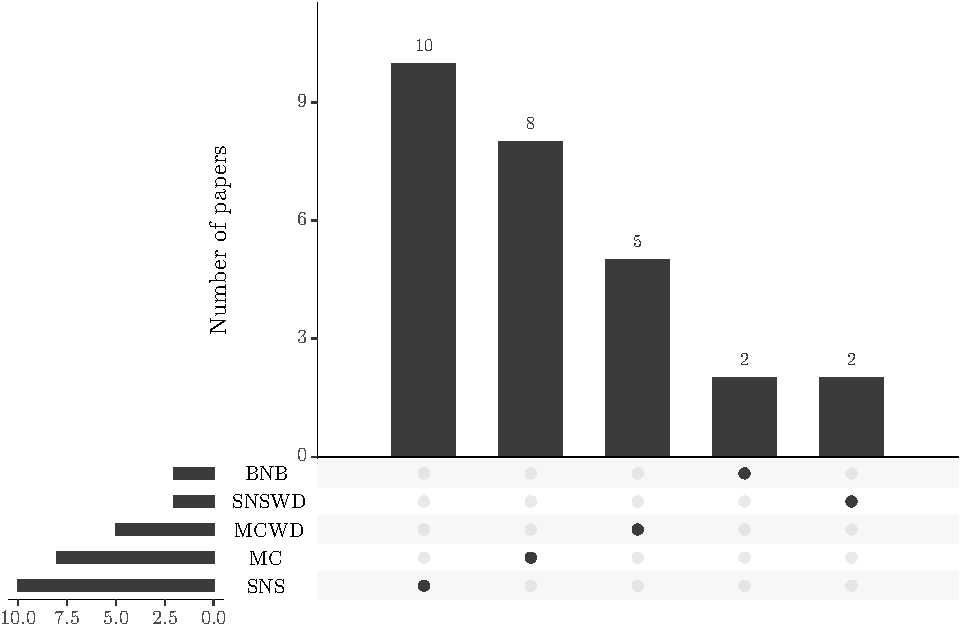
\includegraphics[width=\textwidth]{figures/distribution-by-problem-category-in-ups.pdf}
    \caption{}
    \label{fig:distribution_by_problem-category_in_ups}
  \end{subfigure}\hfill
  \begin{subfigure}{.49\textwidth}
    \centering
    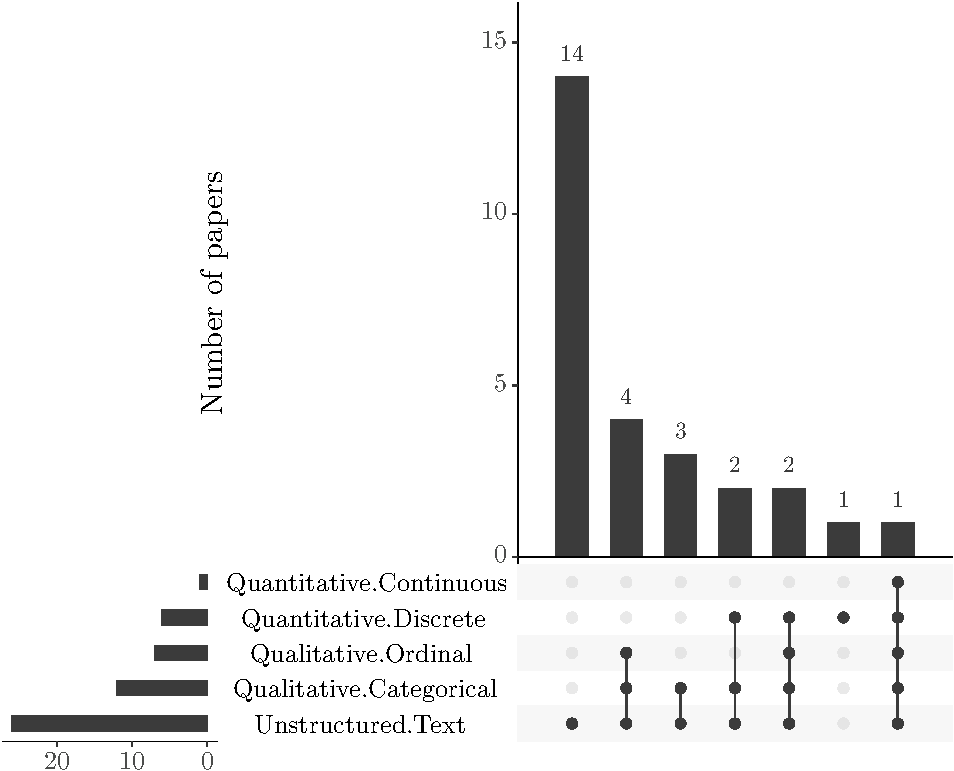
\includegraphics[width=\textwidth]{figures/distribution-by-feature-category-in-ups.pdf}
    \caption{}
    \label{fig:distribution_by_feature_category} 
  \end{subfigure}\hfill
  \begin{subfigure}{.49\textwidth}
    \centering
    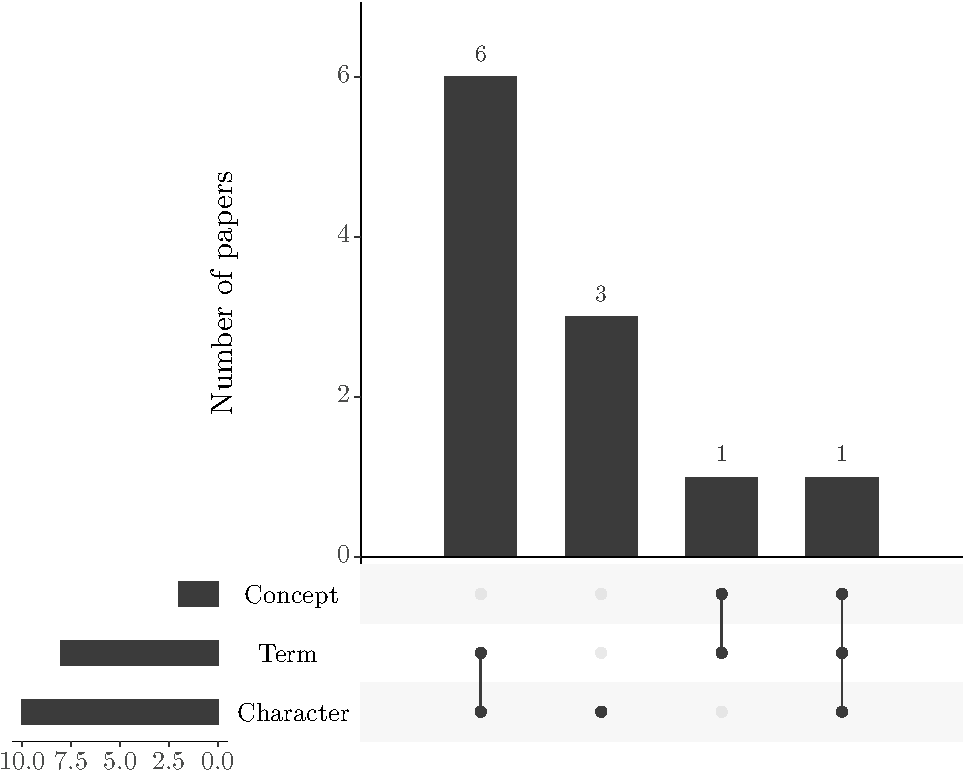
\includegraphics[width=\textwidth]{figures/distribution-by-tm-method-category-in-ups.pdf}
    \caption{}
    \label{fig:distribution-by-tm-method-category}
  \end{subfigure}\hfill
  \begin{subfigure}{.49\textwidth}
    \centering
    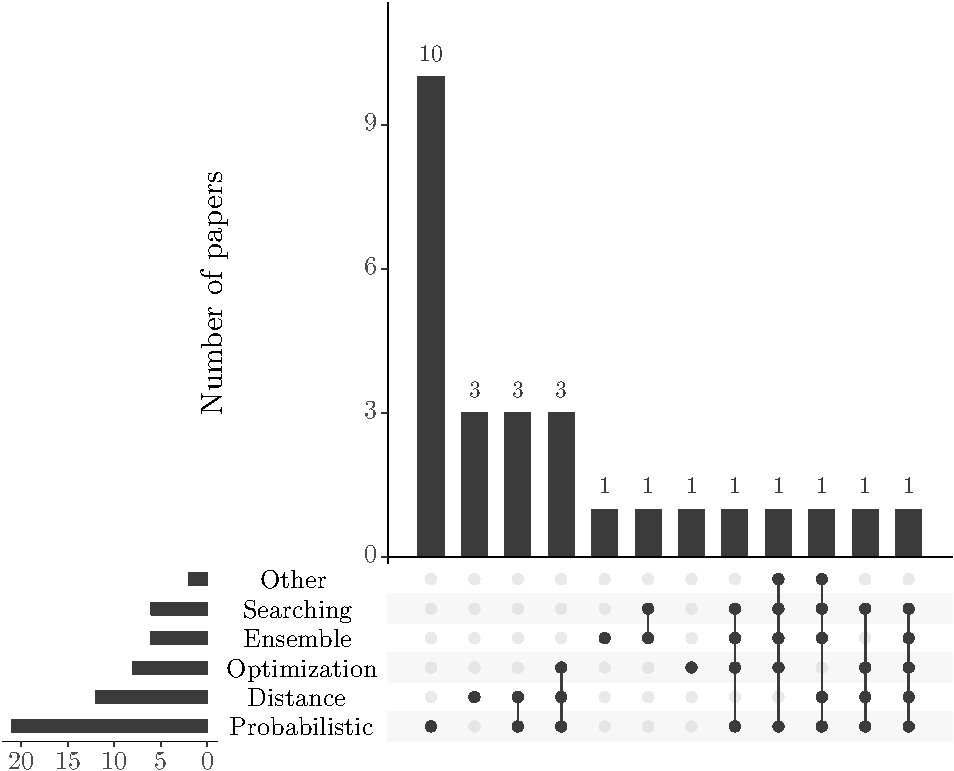
\includegraphics[width=\textwidth]{figures/distribution-by-ml-algorithm-category-in-ups.pdf}
    \caption{}
    \label{fig:distribution-by-ml-algorithm-category} 
  \end{subfigure}
  \caption{(a) Paper distribution by prediction problem category, (b) paper distribution by feature data category, (c) paper distribution by text mining method category (d) paper distribution by ML algorithm categories.}
  \label{fig:rq3_4_6_7_charts}
\end{figure}

\subsection{What are the measures used to evaluate ML algorithms performance for bug report severity prediction (RQ8)?}\label{subsec:rq8_result}

Most papers evaluated the ML model accuracy in bug report severity prediction using three measures based on the confusion matrix (Table~\ref{tab:evaluation_measures_by_papers}): precision ($\approx$ 77\%), recall ($\approx$ 70\%), and f-measure ($\approx$ 66\%). The majority of the used measures are of the single class category (21 out of 27 $\approx$ 70\%), as shown in Figure \ref{fig:distribution_by_evaluation_measure_category}. Only one paper (Roy et al.\cite{Roy:2014}) investigated all four categories of measures presented in the chart.

\begin{table*}[h!]
  \centering
  \captionsetup{type=table}\textsl{}
  \caption{Papers distribution by evaluation measures.}
  \begin{tabular}{@{}llp{8cm}r@{}}
    \toprule
    \textbf{Measure} & \textbf{Category} & \textbf{References} & \textbf{Total} \\
    \midrule
    Precision & Single Class & \cite{Lamkanfi:2010},\cite{Tian:2012},\cite{Chaturvedi:2012},\cite{Yang:2014b},\cite{Valdivia:2014},\cite{Meera:2014},\cite{Roy:2014},\cite{Zhang:2015},\cite{Sharma:2015},\cite{Xia:2015},\cite{Gujral:2015},\cite{Pushpalathas:2016},\cite{Sabor:2016},\cite{Zhang:2016},\cite{Jin:2016a},\cite{Choeikiwong:2016},\cite{Jin:2016b},\cite{Jin:2016c},\cite{Yang:2017},\cite{Singh:2017},\cite{Roy:2017} & 21 \\
    \midrule
    Recall & Single Class & \cite{Lamkanfi:2010},\cite{Tian:2012},\cite{Chaturvedi:2012},\cite{Yang:2014b},\cite{Valdivia:2014},\cite{Meera:2014},\cite{Roy:2014},\cite{Zhang:2015},\cite{Xia:2015},\cite{Pushpalathas:2016},\cite{Sabor:2016},\cite{Zhang:2016},\cite{Jin:2016a},\cite{Choeikiwong:2016},\cite{Jin:2016b},\cite{Jin:2016c},\cite{Yang:2017},\cite{Singh:2017},\cite{Roy:2017} & 19 \\
    \midrule
    F-measure & Single Class & \cite{Lamkanfi:2010},\cite{Tian:2012},\cite{Chaturvedi:2012},\cite{Yang:2014b},\cite{Valdivia:2014},\cite{Meera:2014},\cite{Roy:2014},\cite{Zhang:2015},\cite{Xia:2015},\cite{Sabor:2016},\cite{Zhang:2016},\cite{Jin:2016a},\cite{Choeikiwong:2016},\cite{Jin:2016b},\cite{Jin:2016c},\cite{Yang:2017},\cite{Singh:2017},\cite{Roy:2017} & 18 \\
    \midrule
    Accuracy & Multi-Class & \cite{Chaturvedi:2012},\cite{Yang:2014b},\cite{Valdivia:2014},\cite{Meera:2014},\cite{Roy:2014},\cite{Saha:2015},\cite{Sharma:2015},\cite{Gujral:2015},\cite{Pushpalathas:2016},\cite{Otoom:2016},\cite{Singh:2017} & 11 \\
    \midrule
    AUC & Summary & \cite{Lamkanfi:2010},\cite{Lamkanfi:2011},\cite{Yang:2012},\cite{Yang:2014a},\cite{Roy:2014} & 5 \\
    \midrule
    ROC & Graphical & \cite{Lamkanfi:2010},\cite{Roy:2014} & 2 \\
    \midrule
    MRR\footnotemark & Single Class & \cite{Yang:2014b},\cite{Zhang:2016} & 2 \\
    \midrule
    Effectiveness Ratio\footnotemark & Single Class & \cite{Xia:2015} & 1 \\
    \midrule
    Krippendorff's Alpha Reliability\footnotemark & Single Class & \cite{Tian:2016} & 1 \\
    \bottomrule
  \end{tabular}
  \label{tab:evaluation_measures_by_papers}
\end{table*}
\footnotetext[14]{Mean Reciprocal Rank (MRR)\cite{Zhou:2012} is the average of reciprocal ranks of results of a set of questions. A reciprocal rank of a question is the multiplicative inverse of the rank of the first correct answer.}
\footnotetext[15]{Effectiveness Ratio\cite{Xia:2015} is a cost-effectiveness measure, which evaluates prediction performance given a cost limit.}
\footnotetext[16]{Krippendorff's Alpha Coefficient\cite{Tian:2016} is a statistical measure of the agreement achieved when coding a set o units analysis of values of a variable.}

\subsection{Which sampling techniques are applied most frequently to generate more reliable predictive performance estimates in severity prediction of a bug report (RQ9)?}\label{subsec:rq9_result}

Most papers shown in Table~\ref{tab:sampling_methods_by_papers} applied 10-Fold CV ($\approx$ 66\%) to generate more reliable effectiveness estimates. Figure \ref{fig:distribution_by_sampling_method_category} displays that the majority of those papers (14 out of 15 $\approx$ 93\%) employed a simple resampling method. Also, only one paper (Otoom et al.\cite{Otoom:2016}) investigated both non-resampling and simple resampling methods for bug report severity prediction. 

\begin{table*}[h!]
  \centering
  \captionsetup{type=table}
  \caption{Paper distribution by sampling methods.}
  \small
  \begin{tabular}{@{}llp{8cm}r@{}}
    \toprule
    \textbf{Method} & \textbf{Category} & \textbf{References} & \textbf{Total} \\
    \midrule
    10-Fold CV & Simple Re-sampling & \cite{Lamkanfi:2011},\cite{Yang:2012},\cite{Chaturvedi:2012},\cite{Yang:2014a},\cite{Xia:2015},\cite{Pushpalathas:2016},\cite{Otoom:2016},\cite{Jin:2016b},\cite{Yang:2017},\cite{Roy:2017} & 10 \\
    \midrule
    Stratified 10-Fold CV\footnotemark & Simple Re-sampling & \cite{Valdivia:2014},\cite{Roy:2014},\cite{Singh:2017} & 3 \\
    \midrule
    SMOTE\footnotemark & Simple Re-sampling & \cite{Xia:2015},\cite{Choeikiwong:2016} & 2 \\
    \midrule
    Hold-out & No Re-sampling & \cite{Otoom:2016} & 1 \\
    \midrule
    03-Fold CV & Simple Re-sampling & \cite{Choeikiwong:2016} & 1 \\
    \midrule
    05-Fold CV & Simple Re-sampling & \cite{Sharma:2015} & 1 \\
    \bottomrule
  \end{tabular} 
  \label{tab:sampling_methods_by_papers}
\end{table*}
\footnotetext[17]{Stratified k-fold CV\cite{Japkowicz:2011} is a k-fold CV variation, which ensures that class distribution is respected in the training and testing sets created at every fold.}
\footnotetext[18]{Synthetic Minority Oversampling TEchnique (SMOTE)\cite{Chawla:2002} is an sampling approach in which the minority class is over-sampled by creating ``synthetic" examples rather than by over-sampling with replacement.}

\subsection{Which statistical tests were used to compare the performance between two or more ML algorithms for bug report severity prediction (RQ10)?}\label{subsec:rq10}

As shown in Table~\ref{tab:statistical_test_type_by_papers}, most of the papers used  Wilcoxon Signed Rank Test (8 out of 27 $\approx$ 29\%) and t-test (7 out of 27 - $\approx$ 26\%) to compare the performance of ML algorithms. Figure \ref{fig:distribution-by-statistical-method-category} calls attention that only ten papers ($\approx$ 37\%) reported using any statistical test in their experiments to bug report severity prediction. The figure also shows that most of these papers  (8 out of 10 $\approx$ 80\%) applied a non-parametric test, and 5 out of 10 (50\%) papers employed both parametric and non-parametric tests.  

\begin{table*}[h!]
  \centering
  \captionsetup{type=table}
  \caption{Paper distribution by statistical tests.}
  \begin{tabular}{@{}llp{6cm}r@{}}
    \toprule
    \textbf{Test} & \textbf{Category} & \textbf{References} & \textbf{Total} \\
    \midrule
    Wilcoxon signed rank test & Non-parametric & \cite{Yang:2014b},\cite{Valdivia:2014},\cite{Zhang:2015},\cite{Xia:2015},\cite{Zhang:2016},\cite{Jin:2016b},\cite{Yang:2017},\cite{Singh:2017} & 8 \\
    \midrule
    T-test & Parametric & \cite{Yang:2014b},\cite{Zhang:2015},\cite{Zhang:2016},\cite{Choeikiwong:2016},\cite{Jin:2016b},\cite{Yang:2017},\cite{Roy:2017} & 7 \\
    \midrule
    Proportion test & Parametric & \cite{Roy:2017} & 1 \\
    \midrule
    Shapiro-Wilk test & Parametric & \cite{Yang:2017} & 1 \\
    \bottomrule
  \end{tabular} 
  \label{tab:statistical_test_type_by_papers}
\end{table*}

\subsection{Which software tools were used to run bug report severity prediction experiments (RQ11)?}\label{subsec:rq11} 

Most of the papers listed in Table~\ref{tab:software_tools_used_in_papers} used RapidMiner (5 out of 18 $\approx$ 27\%) to run their experiments. However, Figure \ref{fig:distribution_by_software_tool_category} presents a strong predominance of FLOSS over CSS, 13 out of 18  papers ($\approx$ 61\%) executed  FLOSS to perform their experiments. The figure also shows that no paper used both CSS and FLOSS.

\begin{table*}[h!]
  \centering
  \captionsetup{type=table}
  \caption{Paper distribution by software tools.}
  \begin{tabular}{@{}llp{6cm}r@{}}
    \toprule
    \textbf{Tool} & \textbf{Category} & \textbf{References} & \textbf{Total} \\
    \midrule
    RapidMiner & CSS & \cite{Chaturvedi:2012},\cite{Meera:2014},\cite{Sharma:2015},\cite{Gujral:2015},\cite{Singh:2017} & 5 \\
    \midrule
    WEKA & FLOSS & \cite{Lamkanfi:2011},\cite{Xia:2015},\cite{Pushpalathas:2016},\cite{Tian:2016} & 4 \\
    \midrule
    R & FLOSS & \cite{Yang:2014b},\cite{Zhang:2015},\cite{Yang:2017} & 3 \\
    \midrule
    NLTK & FLOSS & \cite{Roy:2014},\cite{Zhang:2016},\cite{Jin:2016b} & 3 \\
    \midrule
    Statisca & CSS & \cite{Chaturvedi:2012},\cite{Meera:2014} & 2 \\
    \midrule
    TMT & FLOSS & \cite{Yang:2014b},\cite{Zhang:2016} & 2 \\
    \midrule
    OpenNLP & FLOSS & \cite{Tian:2012} & 1 \\
    \midrule
    WordNet & FLOSS & \cite{Roy:2014} & 1 \\
    \midrule
    Ruby & FLOSS & \cite{Lamkanfi:2010} & 1 \\
    \midrule
    WVTool & FLOSS & \cite{Yang:2012} & 1 \\
    \midrule
    CoreNLP & FLOSS & \cite{Yang:2017} & 1 \\
    \bottomrule
  \end{tabular} 
  \label{tab:software_tools_used_in_papers}
\end{table*}

\begin{figure}[!htp]
  \begin{subfigure}{.49\textwidth}
    \centering
    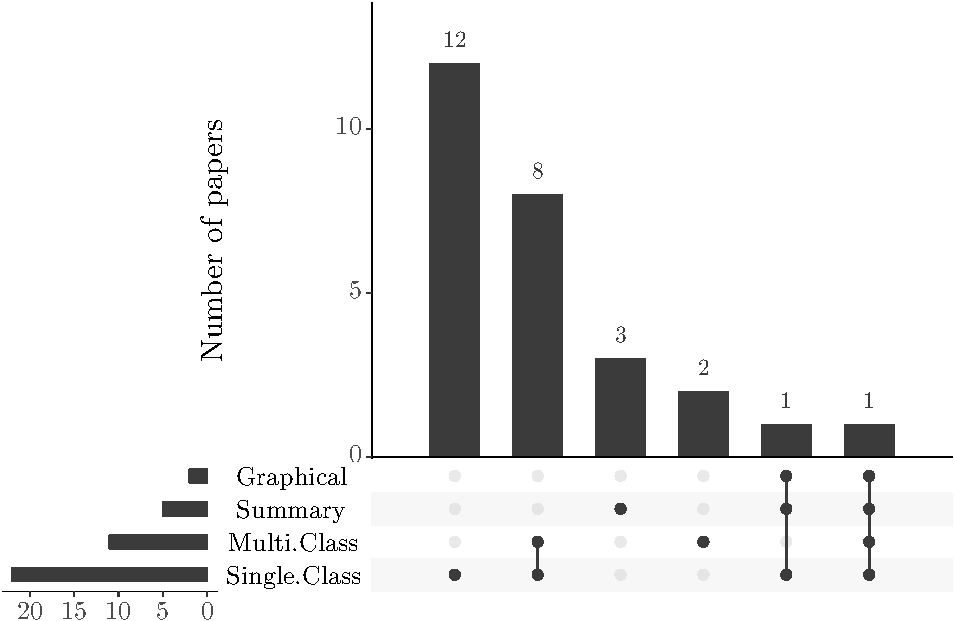
\includegraphics[width=\textwidth]{figures/distribution-by-evaluation-measure-category-in-ups.pdf}
    \caption{}
    \label{fig:distribution_by_evaluation_measure_category}
  \end{subfigure}\hfill
  \begin{subfigure}{.49\textwidth}
    \centering
    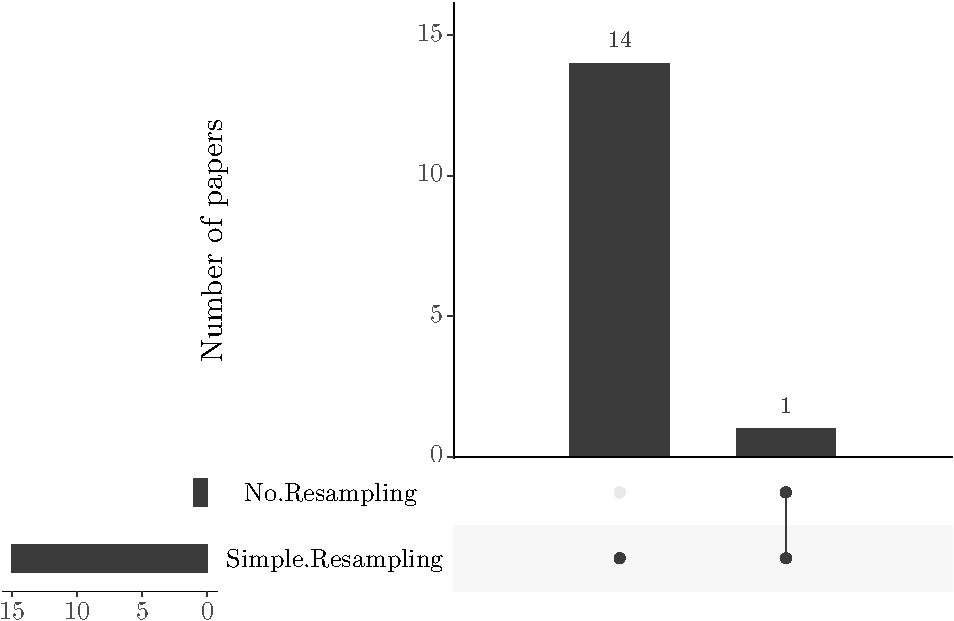
\includegraphics[width=\textwidth]{figures/distribution-by-sampling-method-category-in-ups.pdf}
    \caption{} 
    \label{fig:distribution_by_sampling_method_category}
  \end{subfigure}\hfill
  \begin{subfigure}{.49\textwidth}
    \centering
    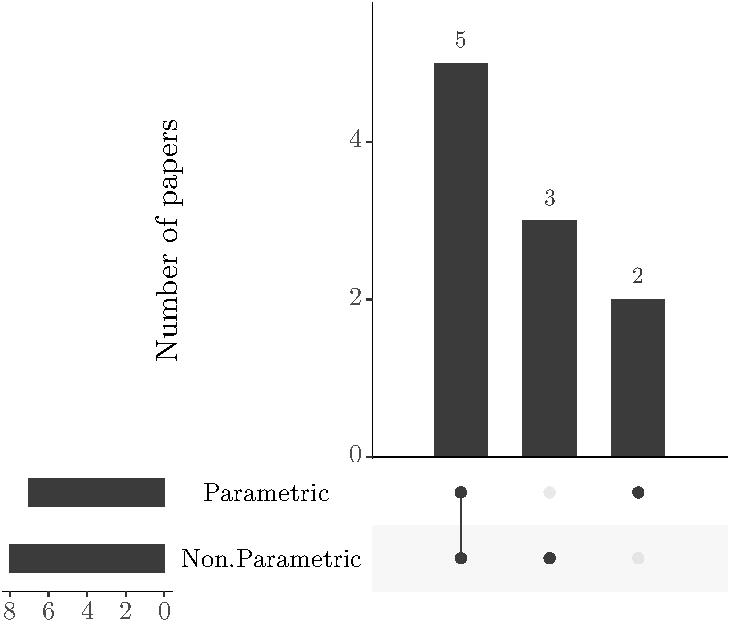
\includegraphics[width=\textwidth]{figures/distribution-by-statistical-method-category-in-ups.pdf}
    \caption{}
    \label{fig:distribution-by-statistical-method-category}
  \end{subfigure}\hfill
  \begin{subfigure}{.49\textwidth}
    \centering
    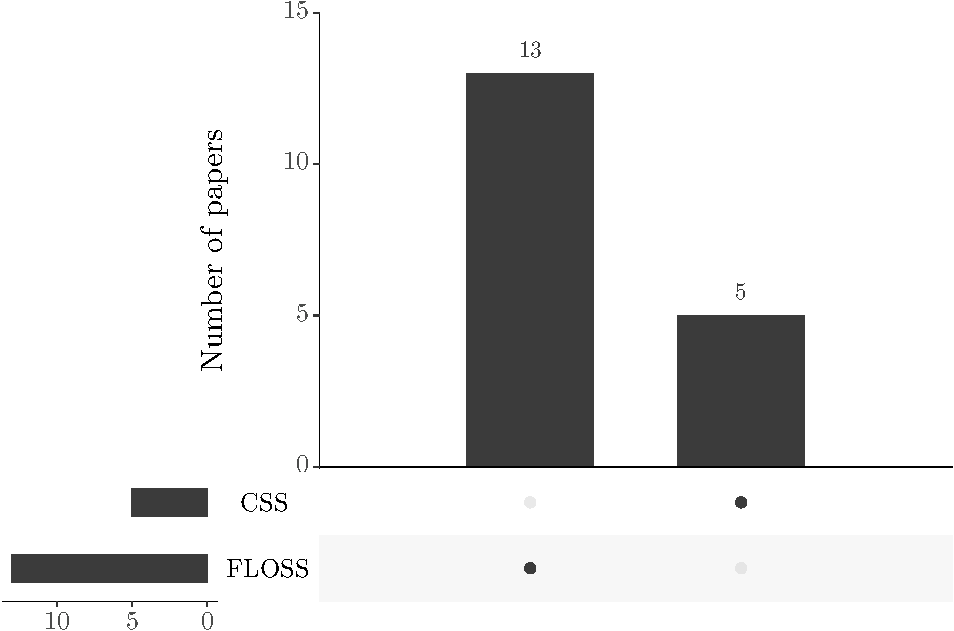
\includegraphics[width=\textwidth]{figures/distribution-by-software-tool-category-in-ups.pdf}
    \caption{}
    \label{fig:distribution_by_software_tool_category} 
  \end{subfigure}
  \caption{(a) Paper distribution by evaluate measure categories, (b) paper distribution by sampling method categories, (c) paper distribution by statistical test categories, and (d) paper distribution by software tool categories.}
  \label{fig:rq8_9_10_11_charts}
\end{figure}
%%%%
\subsection{Which solution types were proposed for bug report severity prediction problem (RQ12)?}\label{subsec:rq12}

Most of the papers (26 out of 27 $\approx$ 93\%) provided offline solutions (Table~\ref{tab:solutions_types_by_papers}). Just one paper (Tian et al. \cite{Tian:2012}) presented an online solution.

\begin{table*}[!htbp]
  \centering
  %\spacebtrows{1.3}
  \caption{Solution types proposed in selected papers.}
  \begin{tabular}{@{}lp{6cm}r@{}}
    \toprule
    Tool & References & Total \\
    \midrule
    offline & \cite{Lamkanfi:2010},\cite{Lamkanfi:2011},\cite{Yang:2012},\cite{Chaturvedi:2012},\cite{Yang:2014b},\cite{Yang:2014a},\cite{Valdivia:2014},\cite{Meera:2014},\cite{Roy:2014},\cite{Saha:2015},\cite{Zhang:2015},\cite{Sharma:2015},\cite{Xia:2015},\cite{Gujral:2015},\cite{Pushpalathas:2016},\cite{Otoom:2016},\cite{Sabor:2016},\cite{Tian:2016},\cite{Zhang:2016},\cite{Jin:2016a},\cite{Choeikiwong:2016},\cite{Jin:2016b},\cite{Jin:2016c},\cite{Yang:2017},\cite{Singh:2017},\cite{Roy:2017} & 26 \\
    \midrule
    online & \cite{Tian:2012} & 1 \\
    \bottomrule
  \end{tabular}
  \label{tab:solutions_types_by_papers}
\end{table*}

\section{Discussion}\label{sec:discussion}
This section presents lessons learned from this systematic mapping study and recommends possible research directions for the bug severity prediction problem.

% RQ2
Researchers have concentrated their focus on few FLOSS, namely Eclipse and Mozilla, both hosted by Bugzilla. The main reason given by most researchers is benchmarking their results with Lamkanfi et al.\cite{Lamkanfi:2010, Lamkanfi:2011}, which are often considered the state-of-the-art in this research area. Notably, they have not considered relevant FLOSS projects like as Linux Kernel, Spark, MySQL, among others. Moreover, published research only marginally investigated two other bug trackers mentioned in reviewed papers: Jira and Google Issue Tracker. The first one tracks bugs for more than 80\% Apache Foundation's projects\footnote[18]{\url{http://www.apache.org/index.html\#projects-list} (As of September 2018).}, and the last one tracks bugs for many internal and external Google Inc. projects\footnote[19]{\url{https://developers.google.com/issue-tracker/} (As of September 2018).}. Surprisingly, for example, no paper investigated Github, another outstanding collaborative website which hosted more than 67 million projects (including many FLOSS)\footnote[20]{\url{https://octoverse.github.com/} (As of September 2018)}.

From 14 FLOSS identified in this review, six are programming tools, four are system software, and four are application software. For former two, people who report bugs are typically technical users, and, for the latter, people are end-users. A bug report can be more or less detailed depending on who reports it\cite{Lamkanfi:2010}\cite{Lamkanfi:2011}. Therefore, the probability of writing more accurate bug reports is larger for technical users than end-users. 

%RQ3
Researchers considered the bug report severity prediction using five different approaches: three of them (SNS, SNSWB, and BNB) predict the severity level from two or three class (coarse-grained). Two other approaches (MC and MCWD) seem to be more complex than problems of the previous ones because the severity level may be predicted from five or six classes (fine-grained). 

From another aspect, two categories (SNSWD and MCWD) did not consider the default severity level (in Bugzilla, often ``normal"). By doing so, they have argued that they would avoid noisy and unreliable data. Saha et al\cite{Saha:2015} confirmed that many bug reports in practice are not ``normal" and this misclassification can really affect the accuracy of ML algorithms.

%RQ4  
Most of the approaches proposed by researchers to predict bug report severity relied on unstructured text features (\textit{summary} and \textit{description}). Because of this, text mining techniques played, side by side with machine learning methods, an essential role in delivering appropriated solutions. Two other features (\textit{product} and \textit{component}) was also quite used in these approaches. That may indicate that bug reports collected from separate parts of a single FLOSS yield different ML algorithms outcomes.

Regarding available feature data types in bug reports, more than half of them are qualitative. SVM and Neural Networks, two popular and essential ML algorithms in modern machine learning\cite{Marsland:2014}, do not work with qualitative data\cite{Flach:2012}. These two facts bring an extra challenge to use qualitative features for bug report severity prediction. When the input data set has qualitative data,  categorical, and ordinal values must be converted into numeric values before applying ML algorithms.

%RQ5
Despite a large number of features raised by the application of text mining activities (e.g., tokenizing, stop word removal and stemming) on \textit{summary} and \textit{description} and of its effectiveness in SNS and SNSWD problems\cite{Yang:2012}, few papers employed feature selection methods for bug severity prediction. Furthermore, these papers notably only investigated filter feature selection methods. Filter-based approaches have two drawbacks\cite{Flach:2012}: (i) they do not take into account redundancy between features, and (ii) they do not detect dependencies between them. 

%RQ6 
Most papers reported the use of unigram for feature extraction. However, few papers explicitly report the use of another text ming methods. Among these papers, the most used method feature vector weighting was TF-IDF and the most used method for verifying text similarity was BM25.


%RQ7
It seems that researchers have adopted a conservative approach regarding the use of ML algorithms. Most papers applied at least one of the following well-known and traditional supervised algorithms: k-NN, Näive Bayes, and its extension Näive Bayes Multinomial.

%RQ8
Researchers evaluated the performance of ML algorithms in their proposed approaches using precision, recall, and f-Measure. Three common measures employed in ML arena, but which may strongly skew in the imbalanced scenario\cite{Jeni:2013}. This characteristic is particularly critical in bug report repositories which are intrinsically imbalanced in practice\cite{Roy:2017}. To minimize such distortion, Tian et al.\cite{Tian:2016}, instead, recommend measuring performance using inter-rater agreement based metrics, such as Cohen's Kappa\cite{Ben-David:2008} or Krippendorff's Alpha\cite{Krippendorff:2011}. Despite its well-known issues in an imbalanced dataset\cite{Japkowicz:2011}, quite few papers still used accuracy to measure ML performance. AUC, an alternative used by few papers, seems more robust than accuracy in imbalanced data conditions. Like Kappa and Krippendorff's Alpha, AUC considers class distribution on performance evaluation of ML algorithms for bug report severity prediction.


%RQ9
Few papers reported the use of a resampling approach to improving the accuracy of ML algorithms. The papers only reported the use of simple resampling strategies, including, the most used, k-fold cross-validation. Only one paper used SMOTE, considered a ``de facto" resampling method in imbalanced data scenario\cite{Fernandez:2018}. Japkowicz et el.\cite{Japkowicz:2011} also suggest that experiments may achieve better results using multiple resampling methods, for example, repeated k-fold cross-validation.

%R10
It seems that most researchers compared the results yielded in their experiments with others observing only the means of measures applied. Few of them reported utilizing statistical tests to do that, which is a recommended practice in empirical software engineering\cite{Kitchenham:2017}. Most used statistical test was parametric.  This kind of test requires that samples follow a statistical distribution (e.g., normal), which is not guaranteed to occur in practice when comparing ML models\cite{Facelli:2015}. Besides, no paper investigated Analysis of Variance (ANOVA), a robust ranked-based test recommended by Kitchenham et al.\cite{Kitchenham:2017} for Empirical Sofware Engineering. 

%R11
Researchers preferred to use FLOSS tools to perform their analyses. Although, many papers have used a proprietary software named RapidMiner. Interestingly, researchers demonstrated a low interest in top-ranked ML tools based on R and Python programming languages.

%R12
It seems that most proposed solutions for bug report severity prediction were conceived to run in offline mode, just one paper claimed which the published solution is mature and fast enough to be embedded, for example, in a web browser. The need for a high number of labeled bug reports during the training phase\cite{Nigam:2012} is a problem intrinsic to supervised ML algorithms, which may make it difficult to turn these offline solutions to online. 
\section{Conclusions and Research Directions}\label{sec:conclusions}

A systematic mapping review provides a structure for a research report type, which enables categorizing and giving a visual summary of results that have been published in papers of a research area\cite{Petersen:2008}. This map aids to identify gaps in a research area, becoming a basis to guide new research activities\cite{Kitchenham:2007}. The current mapping review captured the current state of research on bug report severity prediction, characterized related problems and identified the main approaches employed to solve them. These objectives were reached by conducting a mapping of existing literature. In total, the review identified 27 relevant papers and analyzed them along 12 dimensions. Although these papers have made valuable contributions in bug report severity prediction, the panorama presented in this mapping review suggests that there are potential research opportunities for further improvements in this topic. Among them, the following research directions appear to be more promising:

\begin{itemize}
  \item There is an apparent lack of investigation on bug report severity prediction in other relevant FLOSS such as, for example, Linux Kernel, Ubuntu Linux, and MySQL, and in others BTS, for example, Github.
  \item Often, technical users report most bugs. Thus, the influence of user experience in predicting outcomes is still overlooked.  
  \item Bug reports labeled with default severity level (often ``normal") were prevalent in the most datasets used in reviewed papers. However, they are considered unreliable\cite{Saha:2015}, and just discarding them also does not seem appropriate. Then, efforts in researching on novel approaches to handle this type of report should be considered to improve the state-of-the-art of severity prediction algorithms.
  \item Most approaches were based on unstructured text features (\textit{summary} and \textit{description}). To handle them, researchers chose to use the traditional bag-of-words approach instead of more recent text mining methods (e.g., word-embedding\cite{Guoyin:2018}) or data-driven feature engineering methods which may likely improve outcomes yielded so far.
  \item There is a clear research opportunity to investigate whether state-of-the-art ML algorithms might outperform the traditional algorithms used in all reviewed papers for bug report severity prediction. The investigation of the use of Deep learning algorithms which perform very well when classifying audio, text, and image data\cite{Goodfellow:2016} seems to be a promising research direction.
  \item Researchers should investigate more recent techniques (e.g., continuous learning\cite{Chen:2016}) to provide an approach for bug report prediction which could be employed in real-world scenarios.
  \item Many bug reports are resolved in a few days (or in a few hours)\cite{Saha:2015b}. Efforts to predict severity level for these group of bug reports do not seem very useful. Thus, an investigation to confirm this hypothesis and to determine when the severity prediction is more appropriate in bug report lifecycle is of critical importance.
\end{itemize}

\section*{Acknowledgment}
(omitted for double-blind reviewing). 


\bibliographystyle{IEEEtran}
\bibliography{references}

\end{document}